\documentclass[twoside]{book}

% Packages required by doxygen
\usepackage{fixltx2e}
\usepackage{calc}
\usepackage{doxygen}
\usepackage[export]{adjustbox} % also loads graphicx
\usepackage{graphicx}
\usepackage[utf8]{inputenc}
\usepackage{makeidx}
\usepackage{multicol}
\usepackage{multirow}
\PassOptionsToPackage{warn}{textcomp}
\usepackage{textcomp}
\usepackage[nointegrals]{wasysym}
\usepackage[table]{xcolor}

% Font selection
\usepackage[T1]{fontenc}
\usepackage[scaled=.90]{helvet}
\usepackage{courier}
\usepackage{amssymb}
\usepackage{sectsty}
\renewcommand{\familydefault}{\sfdefault}
\allsectionsfont{%
  \fontseries{bc}\selectfont%
  \color{darkgray}%
}
\renewcommand{\DoxyLabelFont}{%
  \fontseries{bc}\selectfont%
  \color{darkgray}%
}
\newcommand{\+}{\discretionary{\mbox{\scriptsize$\hookleftarrow$}}{}{}}

% Page & text layout
\usepackage{geometry}
\geometry{%
  a4paper,%
  top=2.5cm,%
  bottom=2.5cm,%
  left=2.5cm,%
  right=2.5cm%
}
\tolerance=750
\hfuzz=15pt
\hbadness=750
\setlength{\emergencystretch}{15pt}
\setlength{\parindent}{0cm}
\setlength{\parskip}{3ex plus 2ex minus 2ex}
\makeatletter
\renewcommand{\paragraph}{%
  \@startsection{paragraph}{4}{0ex}{-1.0ex}{1.0ex}{%
    \normalfont\normalsize\bfseries\SS@parafont%
  }%
}
\renewcommand{\subparagraph}{%
  \@startsection{subparagraph}{5}{0ex}{-1.0ex}{1.0ex}{%
    \normalfont\normalsize\bfseries\SS@subparafont%
  }%
}
\makeatother

% Headers & footers
\usepackage{fancyhdr}
\pagestyle{fancyplain}
\fancyhead[LE]{\fancyplain{}{\bfseries\thepage}}
\fancyhead[CE]{\fancyplain{}{}}
\fancyhead[RE]{\fancyplain{}{\bfseries\leftmark}}
\fancyhead[LO]{\fancyplain{}{\bfseries\rightmark}}
\fancyhead[CO]{\fancyplain{}{}}
\fancyhead[RO]{\fancyplain{}{\bfseries\thepage}}
\fancyfoot[LE]{\fancyplain{}{}}
\fancyfoot[CE]{\fancyplain{}{}}
\fancyfoot[RE]{\fancyplain{}{\bfseries\scriptsize Generated by Doxygen }}
\fancyfoot[LO]{\fancyplain{}{\bfseries\scriptsize Generated by Doxygen }}
\fancyfoot[CO]{\fancyplain{}{}}
\fancyfoot[RO]{\fancyplain{}{}}
\renewcommand{\footrulewidth}{0.4pt}
\renewcommand{\chaptermark}[1]{%
  \markboth{#1}{}%
}
\renewcommand{\sectionmark}[1]{%
  \markright{\thesection\ #1}%
}

% Indices & bibliography
\usepackage{natbib}
\usepackage[titles]{tocloft}
\setcounter{tocdepth}{3}
\setcounter{secnumdepth}{5}
\makeindex

% Hyperlinks (required, but should be loaded last)
\usepackage{ifpdf}
\ifpdf
  \usepackage[pdftex,pagebackref=true]{hyperref}
\else
  \usepackage[ps2pdf,pagebackref=true]{hyperref}
\fi
\hypersetup{%
  colorlinks=true,%
  linkcolor=blue,%
  citecolor=blue,%
  unicode%
}

% Custom commands
\newcommand{\clearemptydoublepage}{%
  \newpage{\pagestyle{empty}\cleardoublepage}%
}

\usepackage{caption}
\captionsetup{labelsep=space,justification=centering,font={bf},singlelinecheck=off,skip=4pt,position=top}

%===== C O N T E N T S =====

\begin{document}

% Titlepage & ToC
\hypersetup{pageanchor=false,
             bookmarksnumbered=true,
             pdfencoding=unicode
            }
\pagenumbering{alph}
\begin{titlepage}
\vspace*{7cm}
\begin{center}%
{\Large Access Controll Logging Tool \\[1ex]\large V1.\+0.\+3 }\\
\vspace*{1cm}
{\large Generated by Doxygen 1.8.13}\\
\end{center}
\end{titlepage}
\clearemptydoublepage
\pagenumbering{roman}
\tableofcontents
\clearemptydoublepage
\pagenumbering{arabic}
\hypersetup{pageanchor=true}

%--- Begin generated contents ---
\chapter{Assignment 2}
\label{md_README}
\Hypertarget{md_README}
\subsection*{Access Controll Logging Tool}

\subsubsection*{Description}

The access controll logging system monitors and keeps track of every file access and modification that occurs in the system.

\begin{quote}
\+:warning\+:

Systemwide logging can throw errors (notably in the case of \textquotesingle{}gcc\textquotesingle{}) that are not related to the program itself, but to the nature of the temp files these commands use.

\begin{quote}


It is best to disable the preloading before running these commands. \end{quote}
\end{quote}


\subsubsection*{Compilation}

to compile the program, run the following command in the root directory of the project\+:


\begin{DoxyCode}
make clean
make
\end{DoxyCode}


\subsubsection*{Execution}

the program runs in the backround. The systemwide can be enabled and disabled using the following commands\+:


\begin{DoxyCode}
LD\_PRELOAD=./out/libmylib.so    // Enables the logging
LD\_PRELOAD=                     // Disables the logging
\end{DoxyCode}


\subsubsection*{Testing}

The program can be tested with the following commands\+:


\begin{DoxyCode}
make test
\end{DoxyCode}
 
\chapter{Data Structure Index}
\section{Data Structures}
Here are the data structures with brief descriptions\+:\begin{DoxyCompactList}
\item\contentsline{section}{\hyperlink{structlog__entry}{log\+\_\+entry} }{\pageref{structlog__entry}}{}
\item\contentsline{section}{\hyperlink{structlog__entry__text__hash}{log\+\_\+entry\+\_\+text\+\_\+hash} }{\pageref{structlog__entry__text__hash}}{}
\end{DoxyCompactList}

\chapter{File Index}
\section{File List}
Here is a list of all files with brief descriptions\+:\begin{DoxyCompactList}
\item\contentsline{section}{\hyperlink{ACL_8c}{A\+C\+L.\+c} }{\pageref{ACL_8c}}{}
\item\contentsline{section}{\hyperlink{acmonitor_8c}{acmonitor.\+c} }{\pageref{acmonitor_8c}}{}
\item\contentsline{section}{\hyperlink{fhandler_8c}{fhandler.\+c} }{\pageref{fhandler_8c}}{}
\item\contentsline{section}{\hyperlink{fhandler_8h}{fhandler.\+h} }{\pageref{fhandler_8h}}{}
\item\contentsline{section}{\hyperlink{fmod__test_8c}{fmod\+\_\+test.\+c} }{\pageref{fmod__test_8c}}{}
\item\contentsline{section}{\hyperlink{fperm__test_8c}{fperm\+\_\+test.\+c} }{\pageref{fperm__test_8c}}{}
\item\contentsline{section}{\hyperlink{log_8c}{log.\+c} }{\pageref{log_8c}}{}
\item\contentsline{section}{\hyperlink{log_8h}{log.\+h} }{\pageref{log_8h}}{}
\item\contentsline{section}{\hyperlink{main_8c}{main.\+c} }{\pageref{main_8c}}{}
\item\contentsline{section}{\hyperlink{Misc_8h}{Misc.\+h} }{\pageref{Misc_8h}}{}
\item\contentsline{section}{\hyperlink{sarray__test_8c}{sarray\+\_\+test.\+c} }{\pageref{sarray__test_8c}}{}
\item\contentsline{section}{\hyperlink{template_8c}{template.\+c} }{\pageref{template_8c}}{}
\item\contentsline{section}{\hyperlink{test__aclog_8c}{test\+\_\+aclog.\+c} }{\pageref{test__aclog_8c}}{}
\end{DoxyCompactList}

\chapter{Data Structure Documentation}
\hypertarget{structlog__entry}{}\section{log\+\_\+entry Struct Reference}
\label{structlog__entry}\index{log\+\_\+entry@{log\+\_\+entry}}


The log entry.  




{\ttfamily \#include $<$log.\+h$>$}

\subsection*{Data Fields}
\begin{DoxyCompactItemize}
\item 
const unsigned int \hyperlink{structlog__entry_a879f3cffed87111c14b5ddca7bf36bfe_a879f3cffed87111c14b5ddca7bf36bfe}{U\+ID}
\item 
const char $\ast$ \hyperlink{structlog__entry_af95c41539cb49570c94f3cdbce83440b_af95c41539cb49570c94f3cdbce83440b}{path}
\item 
const struct tm \hyperlink{structlog__entry_a50022de0184c303275407ebd7eb65c63_a50022de0184c303275407ebd7eb65c63}{timestamp}
\item 
const \hyperlink{log_8h_ab20c54dfb1eb1323b9a3cfe2e6a76270_ab20c54dfb1eb1323b9a3cfe2e6a76270}{access\+\_\+t} \hyperlink{structlog__entry_a36a8d704c97e0fa5f3f83454e2d92662_a36a8d704c97e0fa5f3f83454e2d92662}{access}
\item 
const int \hyperlink{structlog__entry_a7845b16ee2d60f04349b65d55c44dd50_a7845b16ee2d60f04349b65d55c44dd50}{action\+\_\+denied}
\item 
const char \hyperlink{structlog__entry_af2ebb7fded35fda20794591db630571e_af2ebb7fded35fda20794591db630571e}{fingerprint} \mbox{[}33\mbox{]}
\end{DoxyCompactItemize}


\subsection{Detailed Description}
The log entry. 


\begin{DoxyParams}{Parameters}
{\em U\+ID} & The U\+ID of the user. \\
\hline
{\em path} & The absolute path of the file. \\
\hline
{\em timestamp} & The timestamp of the log entry. \\
\hline
{\em access} & The access type. see access\+\_\+t \\
\hline
{\em action\+\_\+denied} & 1 if the action was denied, else 0. \\
\hline
{\em fingerprint} & The fingerprint of the file. \\
\hline
\end{DoxyParams}


\subsection{Field Documentation}
\mbox{\Hypertarget{structlog__entry_a36a8d704c97e0fa5f3f83454e2d92662_a36a8d704c97e0fa5f3f83454e2d92662}\label{structlog__entry_a36a8d704c97e0fa5f3f83454e2d92662_a36a8d704c97e0fa5f3f83454e2d92662}} 
\index{log\+\_\+entry@{log\+\_\+entry}!access@{access}}
\index{access@{access}!log\+\_\+entry@{log\+\_\+entry}}
\subsubsection{\texorpdfstring{access}{access}}
{\footnotesize\ttfamily const \hyperlink{log_8h_ab20c54dfb1eb1323b9a3cfe2e6a76270_ab20c54dfb1eb1323b9a3cfe2e6a76270}{access\+\_\+t} log\+\_\+entry\+::access}

\mbox{\Hypertarget{structlog__entry_a7845b16ee2d60f04349b65d55c44dd50_a7845b16ee2d60f04349b65d55c44dd50}\label{structlog__entry_a7845b16ee2d60f04349b65d55c44dd50_a7845b16ee2d60f04349b65d55c44dd50}} 
\index{log\+\_\+entry@{log\+\_\+entry}!action\+\_\+denied@{action\+\_\+denied}}
\index{action\+\_\+denied@{action\+\_\+denied}!log\+\_\+entry@{log\+\_\+entry}}
\subsubsection{\texorpdfstring{action\+\_\+denied}{action\_denied}}
{\footnotesize\ttfamily const int log\+\_\+entry\+::action\+\_\+denied}

\mbox{\Hypertarget{structlog__entry_af2ebb7fded35fda20794591db630571e_af2ebb7fded35fda20794591db630571e}\label{structlog__entry_af2ebb7fded35fda20794591db630571e_af2ebb7fded35fda20794591db630571e}} 
\index{log\+\_\+entry@{log\+\_\+entry}!fingerprint@{fingerprint}}
\index{fingerprint@{fingerprint}!log\+\_\+entry@{log\+\_\+entry}}
\subsubsection{\texorpdfstring{fingerprint}{fingerprint}}
{\footnotesize\ttfamily const char log\+\_\+entry\+::fingerprint\mbox{[}33\mbox{]}}

\mbox{\Hypertarget{structlog__entry_af95c41539cb49570c94f3cdbce83440b_af95c41539cb49570c94f3cdbce83440b}\label{structlog__entry_af95c41539cb49570c94f3cdbce83440b_af95c41539cb49570c94f3cdbce83440b}} 
\index{log\+\_\+entry@{log\+\_\+entry}!path@{path}}
\index{path@{path}!log\+\_\+entry@{log\+\_\+entry}}
\subsubsection{\texorpdfstring{path}{path}}
{\footnotesize\ttfamily const char$\ast$ log\+\_\+entry\+::path}

\mbox{\Hypertarget{structlog__entry_a50022de0184c303275407ebd7eb65c63_a50022de0184c303275407ebd7eb65c63}\label{structlog__entry_a50022de0184c303275407ebd7eb65c63_a50022de0184c303275407ebd7eb65c63}} 
\index{log\+\_\+entry@{log\+\_\+entry}!timestamp@{timestamp}}
\index{timestamp@{timestamp}!log\+\_\+entry@{log\+\_\+entry}}
\subsubsection{\texorpdfstring{timestamp}{timestamp}}
{\footnotesize\ttfamily const struct tm log\+\_\+entry\+::timestamp}

\mbox{\Hypertarget{structlog__entry_a879f3cffed87111c14b5ddca7bf36bfe_a879f3cffed87111c14b5ddca7bf36bfe}\label{structlog__entry_a879f3cffed87111c14b5ddca7bf36bfe_a879f3cffed87111c14b5ddca7bf36bfe}} 
\index{log\+\_\+entry@{log\+\_\+entry}!U\+ID@{U\+ID}}
\index{U\+ID@{U\+ID}!log\+\_\+entry@{log\+\_\+entry}}
\subsubsection{\texorpdfstring{U\+ID}{UID}}
{\footnotesize\ttfamily const unsigned int log\+\_\+entry\+::\+U\+ID}



The documentation for this struct was generated from the following file\+:\begin{DoxyCompactItemize}
\item 
\hyperlink{log_8h}{log.\+h}\end{DoxyCompactItemize}

\hypertarget{structlog__entry__text__hash}{}\section{log\+\_\+entry\+\_\+text\+\_\+hash Struct Reference}
\label{structlog__entry__text__hash}\index{log\+\_\+entry\+\_\+text\+\_\+hash@{log\+\_\+entry\+\_\+text\+\_\+hash}}
\subsection*{Data Fields}
\begin{DoxyCompactItemize}
\item 
unsigned int \hyperlink{structlog__entry__text__hash_a68c5ad6594b98c96c933705d5d2b6167_a68c5ad6594b98c96c933705d5d2b6167}{U\+ID}
\item 
char $\ast$ \hyperlink{structlog__entry__text__hash_a991fd47833c6a7e56c8b0713ef85870e_a991fd47833c6a7e56c8b0713ef85870e}{path}
\item 
struct tm \hyperlink{structlog__entry__text__hash_af528ed5b63af8fed3be408fdbe36195e_af528ed5b63af8fed3be408fdbe36195e}{timestamp}
\item 
char \hyperlink{structlog__entry__text__hash_a063ec2686e19fb9054ecea7e1bafa171_a063ec2686e19fb9054ecea7e1bafa171}{access} \mbox{[}7\mbox{]}
\item 
int \hyperlink{structlog__entry__text__hash_acd30ad7fd2030eb270130884aa559aa8_acd30ad7fd2030eb270130884aa559aa8}{action\+\_\+denied}
\item 
char \hyperlink{structlog__entry__text__hash_a31ffdc8e1cf0fcaba871975eb56ed4ce_a31ffdc8e1cf0fcaba871975eb56ed4ce}{fingerprint} \mbox{[}33\mbox{]}
\end{DoxyCompactItemize}


\subsection{Field Documentation}
\mbox{\Hypertarget{structlog__entry__text__hash_a063ec2686e19fb9054ecea7e1bafa171_a063ec2686e19fb9054ecea7e1bafa171}\label{structlog__entry__text__hash_a063ec2686e19fb9054ecea7e1bafa171_a063ec2686e19fb9054ecea7e1bafa171}} 
\index{log\+\_\+entry\+\_\+text\+\_\+hash@{log\+\_\+entry\+\_\+text\+\_\+hash}!access@{access}}
\index{access@{access}!log\+\_\+entry\+\_\+text\+\_\+hash@{log\+\_\+entry\+\_\+text\+\_\+hash}}
\subsubsection{\texorpdfstring{access}{access}}
{\footnotesize\ttfamily char log\+\_\+entry\+\_\+text\+\_\+hash\+::access\mbox{[}7\mbox{]}}

\mbox{\Hypertarget{structlog__entry__text__hash_acd30ad7fd2030eb270130884aa559aa8_acd30ad7fd2030eb270130884aa559aa8}\label{structlog__entry__text__hash_acd30ad7fd2030eb270130884aa559aa8_acd30ad7fd2030eb270130884aa559aa8}} 
\index{log\+\_\+entry\+\_\+text\+\_\+hash@{log\+\_\+entry\+\_\+text\+\_\+hash}!action\+\_\+denied@{action\+\_\+denied}}
\index{action\+\_\+denied@{action\+\_\+denied}!log\+\_\+entry\+\_\+text\+\_\+hash@{log\+\_\+entry\+\_\+text\+\_\+hash}}
\subsubsection{\texorpdfstring{action\+\_\+denied}{action\_denied}}
{\footnotesize\ttfamily int log\+\_\+entry\+\_\+text\+\_\+hash\+::action\+\_\+denied}

\mbox{\Hypertarget{structlog__entry__text__hash_a31ffdc8e1cf0fcaba871975eb56ed4ce_a31ffdc8e1cf0fcaba871975eb56ed4ce}\label{structlog__entry__text__hash_a31ffdc8e1cf0fcaba871975eb56ed4ce_a31ffdc8e1cf0fcaba871975eb56ed4ce}} 
\index{log\+\_\+entry\+\_\+text\+\_\+hash@{log\+\_\+entry\+\_\+text\+\_\+hash}!fingerprint@{fingerprint}}
\index{fingerprint@{fingerprint}!log\+\_\+entry\+\_\+text\+\_\+hash@{log\+\_\+entry\+\_\+text\+\_\+hash}}
\subsubsection{\texorpdfstring{fingerprint}{fingerprint}}
{\footnotesize\ttfamily char log\+\_\+entry\+\_\+text\+\_\+hash\+::fingerprint\mbox{[}33\mbox{]}}

\mbox{\Hypertarget{structlog__entry__text__hash_a991fd47833c6a7e56c8b0713ef85870e_a991fd47833c6a7e56c8b0713ef85870e}\label{structlog__entry__text__hash_a991fd47833c6a7e56c8b0713ef85870e_a991fd47833c6a7e56c8b0713ef85870e}} 
\index{log\+\_\+entry\+\_\+text\+\_\+hash@{log\+\_\+entry\+\_\+text\+\_\+hash}!path@{path}}
\index{path@{path}!log\+\_\+entry\+\_\+text\+\_\+hash@{log\+\_\+entry\+\_\+text\+\_\+hash}}
\subsubsection{\texorpdfstring{path}{path}}
{\footnotesize\ttfamily char$\ast$ log\+\_\+entry\+\_\+text\+\_\+hash\+::path}

\mbox{\Hypertarget{structlog__entry__text__hash_af528ed5b63af8fed3be408fdbe36195e_af528ed5b63af8fed3be408fdbe36195e}\label{structlog__entry__text__hash_af528ed5b63af8fed3be408fdbe36195e_af528ed5b63af8fed3be408fdbe36195e}} 
\index{log\+\_\+entry\+\_\+text\+\_\+hash@{log\+\_\+entry\+\_\+text\+\_\+hash}!timestamp@{timestamp}}
\index{timestamp@{timestamp}!log\+\_\+entry\+\_\+text\+\_\+hash@{log\+\_\+entry\+\_\+text\+\_\+hash}}
\subsubsection{\texorpdfstring{timestamp}{timestamp}}
{\footnotesize\ttfamily struct tm log\+\_\+entry\+\_\+text\+\_\+hash\+::timestamp}

\mbox{\Hypertarget{structlog__entry__text__hash_a68c5ad6594b98c96c933705d5d2b6167_a68c5ad6594b98c96c933705d5d2b6167}\label{structlog__entry__text__hash_a68c5ad6594b98c96c933705d5d2b6167_a68c5ad6594b98c96c933705d5d2b6167}} 
\index{log\+\_\+entry\+\_\+text\+\_\+hash@{log\+\_\+entry\+\_\+text\+\_\+hash}!U\+ID@{U\+ID}}
\index{U\+ID@{U\+ID}!log\+\_\+entry\+\_\+text\+\_\+hash@{log\+\_\+entry\+\_\+text\+\_\+hash}}
\subsubsection{\texorpdfstring{U\+ID}{UID}}
{\footnotesize\ttfamily unsigned int log\+\_\+entry\+\_\+text\+\_\+hash\+::\+U\+ID}



The documentation for this struct was generated from the following file\+:\begin{DoxyCompactItemize}
\item 
\hyperlink{acmonitor_8c}{acmonitor.\+c}\end{DoxyCompactItemize}

\chapter{File Documentation}
\hypertarget{ACL_8c}{}\section{A\+C\+L.\+c File Reference}
\label{ACL_8c}\index{A\+C\+L.\+c@{A\+C\+L.\+c}}
{\ttfamily \#include $<$stdio.\+h$>$}\newline
{\ttfamily \#include $<$stdlib.\+h$>$}\newline
{\ttfamily \#include $<$string.\+h$>$}\newline
{\ttfamily \#include $<$dlfcn.\+h$>$}\newline
{\ttfamily \#include $<$errno.\+h$>$}\newline
{\ttfamily \#include $<$unistd.\+h$>$}\newline
{\ttfamily \#include $<$stdarg.\+h$>$}\newline
{\ttfamily \#include $<$openssl/md5.\+h$>$}\newline
{\ttfamily \#include \char`\"{}log.\+h\char`\"{}}\newline
{\ttfamily \#include \char`\"{}fhandler.\+h\char`\"{}}\newline
Include dependency graph for A\+C\+L.\+c\+:\nopagebreak
\begin{figure}[H]
\begin{center}
\leavevmode
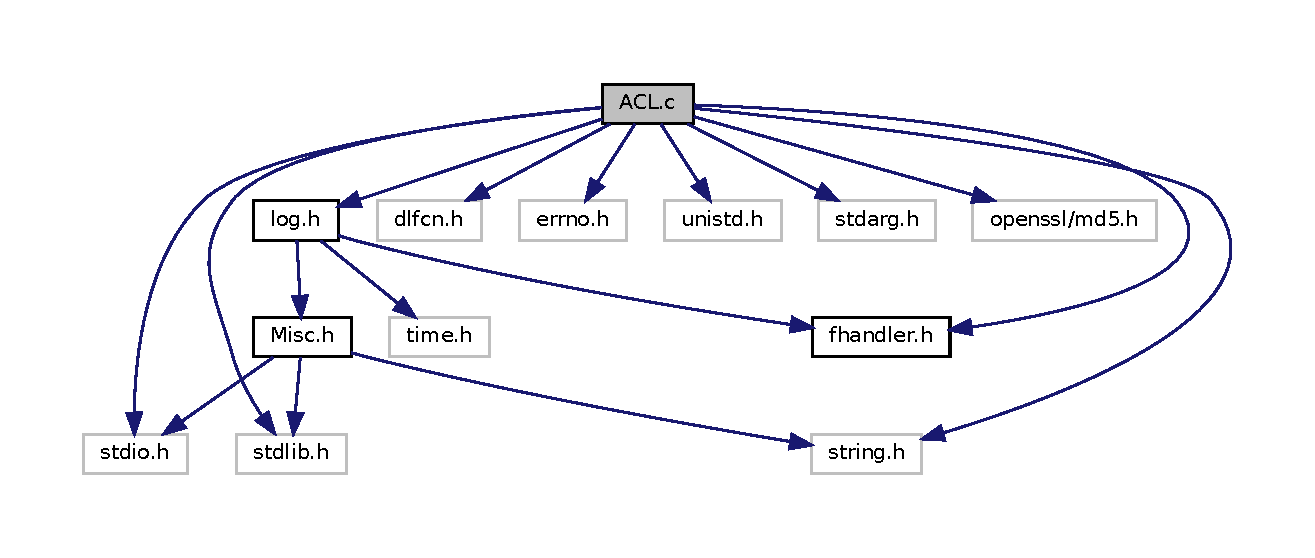
\includegraphics[width=350pt]{ACL_8c__incl}
\end{center}
\end{figure}
\subsection*{Macros}
\begin{DoxyCompactItemize}
\item 
\#define \hyperlink{ACL_8c_a369266c24eacffb87046522897a570d5_a369266c24eacffb87046522897a570d5}{\+\_\+\+G\+N\+U\+\_\+\+S\+O\+U\+R\+CE}
\item 
\#define \hyperlink{ACL_8c_ac4c027058e9ccd1d4dce6a718af0b422_ac4c027058e9ccd1d4dce6a718af0b422}{printd}(format, ...)
\item 
\#define \hyperlink{ACL_8c_a8b3a3c4c8735fffe0d3b0ab6c7053667_a8b3a3c4c8735fffe0d3b0ab6c7053667}{printld}(format, ...)
\item 
\#define \hyperlink{ACL_8c_a483d4c865c4cb956ffe919f48867641a_a483d4c865c4cb956ffe919f48867641a}{printv}(format, ...)
\end{DoxyCompactItemize}
\subsection*{Functions}
\begin{DoxyCompactItemize}
\item 
char $\ast$ \hyperlink{ACL_8c_ae458807f7bf6dc176a3f783da321f6ec_ae458807f7bf6dc176a3f783da321f6ec}{get\+\_\+path} (F\+I\+LE $\ast$f)
\begin{DoxyCompactList}\small\item\em returns the absolute path of a file stream \end{DoxyCompactList}\item 
unsigned char $\ast$ \hyperlink{ACL_8c_a7da6115f144b2d630d5f090399ee4645_a7da6115f144b2d630d5f090399ee4645}{Hash} (F\+I\+LE $\ast$fp)
\begin{DoxyCompactList}\small\item\em Creates a hash key from the contents of a file. \end{DoxyCompactList}\item 
unsigned char $\ast$ \hyperlink{ACL_8c_a4c27f974a9c92361a21efd1bb444e170_a4c27f974a9c92361a21efd1bb444e170}{Hash\+\_\+string} (char $\ast$str)
\begin{DoxyCompactList}\small\item\em Creates a hash key from a string. \end{DoxyCompactList}\end{DoxyCompactItemize}


\subsection{Macro Definition Documentation}
\mbox{\Hypertarget{ACL_8c_a369266c24eacffb87046522897a570d5_a369266c24eacffb87046522897a570d5}\label{ACL_8c_a369266c24eacffb87046522897a570d5_a369266c24eacffb87046522897a570d5}} 
\index{A\+C\+L.\+c@{A\+C\+L.\+c}!\+\_\+\+G\+N\+U\+\_\+\+S\+O\+U\+R\+CE@{\+\_\+\+G\+N\+U\+\_\+\+S\+O\+U\+R\+CE}}
\index{\+\_\+\+G\+N\+U\+\_\+\+S\+O\+U\+R\+CE@{\+\_\+\+G\+N\+U\+\_\+\+S\+O\+U\+R\+CE}!A\+C\+L.\+c@{A\+C\+L.\+c}}
\subsubsection{\texorpdfstring{\+\_\+\+G\+N\+U\+\_\+\+S\+O\+U\+R\+CE}{\_GNU\_SOURCE}}
{\footnotesize\ttfamily \#define \+\_\+\+G\+N\+U\+\_\+\+S\+O\+U\+R\+CE}

\mbox{\Hypertarget{ACL_8c_ac4c027058e9ccd1d4dce6a718af0b422_ac4c027058e9ccd1d4dce6a718af0b422}\label{ACL_8c_ac4c027058e9ccd1d4dce6a718af0b422_ac4c027058e9ccd1d4dce6a718af0b422}} 
\index{A\+C\+L.\+c@{A\+C\+L.\+c}!printd@{printd}}
\index{printd@{printd}!A\+C\+L.\+c@{A\+C\+L.\+c}}
\subsubsection{\texorpdfstring{printd}{printd}}
{\footnotesize\ttfamily \#define printd(\begin{DoxyParamCaption}\item[{}]{format,  }\item[{}]{... }\end{DoxyParamCaption})}

\mbox{\Hypertarget{ACL_8c_a8b3a3c4c8735fffe0d3b0ab6c7053667_a8b3a3c4c8735fffe0d3b0ab6c7053667}\label{ACL_8c_a8b3a3c4c8735fffe0d3b0ab6c7053667_a8b3a3c4c8735fffe0d3b0ab6c7053667}} 
\index{A\+C\+L.\+c@{A\+C\+L.\+c}!printld@{printld}}
\index{printld@{printld}!A\+C\+L.\+c@{A\+C\+L.\+c}}
\subsubsection{\texorpdfstring{printld}{printld}}
{\footnotesize\ttfamily \#define printld(\begin{DoxyParamCaption}\item[{}]{format,  }\item[{}]{... }\end{DoxyParamCaption})}

\mbox{\Hypertarget{ACL_8c_a483d4c865c4cb956ffe919f48867641a_a483d4c865c4cb956ffe919f48867641a}\label{ACL_8c_a483d4c865c4cb956ffe919f48867641a_a483d4c865c4cb956ffe919f48867641a}} 
\index{A\+C\+L.\+c@{A\+C\+L.\+c}!printv@{printv}}
\index{printv@{printv}!A\+C\+L.\+c@{A\+C\+L.\+c}}
\subsubsection{\texorpdfstring{printv}{printv}}
{\footnotesize\ttfamily \#define printv(\begin{DoxyParamCaption}\item[{}]{format,  }\item[{}]{... }\end{DoxyParamCaption})}



\subsection{Function Documentation}
\mbox{\Hypertarget{ACL_8c_ae458807f7bf6dc176a3f783da321f6ec_ae458807f7bf6dc176a3f783da321f6ec}\label{ACL_8c_ae458807f7bf6dc176a3f783da321f6ec_ae458807f7bf6dc176a3f783da321f6ec}} 
\index{A\+C\+L.\+c@{A\+C\+L.\+c}!get\+\_\+path@{get\+\_\+path}}
\index{get\+\_\+path@{get\+\_\+path}!A\+C\+L.\+c@{A\+C\+L.\+c}}
\subsubsection{\texorpdfstring{get\+\_\+path()}{get\_path()}}
{\footnotesize\ttfamily char$\ast$ get\+\_\+path (\begin{DoxyParamCaption}\item[{F\+I\+LE $\ast$}]{f }\end{DoxyParamCaption})}



returns the absolute path of a file stream 


\begin{DoxyParams}{Parameters}
{\em f} & The file stream \\
\hline
\end{DoxyParams}
\begin{DoxyReturn}{Returns}
char$\ast$ The absolute path of the file stream
\end{DoxyReturn}
\begin{DoxyWarning}{Warning}
This function is not tested.
\end{DoxyWarning}
\begin{DoxyRefDesc}{Todo}
\item[\hyperlink{todo__todo000002}{Todo}]test this function \end{DoxyRefDesc}
\mbox{\Hypertarget{ACL_8c_a7da6115f144b2d630d5f090399ee4645_a7da6115f144b2d630d5f090399ee4645}\label{ACL_8c_a7da6115f144b2d630d5f090399ee4645_a7da6115f144b2d630d5f090399ee4645}} 
\index{A\+C\+L.\+c@{A\+C\+L.\+c}!Hash@{Hash}}
\index{Hash@{Hash}!A\+C\+L.\+c@{A\+C\+L.\+c}}
\subsubsection{\texorpdfstring{Hash()}{Hash()}}
{\footnotesize\ttfamily unsigned char$\ast$ Hash (\begin{DoxyParamCaption}\item[{F\+I\+LE $\ast$}]{fp }\end{DoxyParamCaption})}



Creates a hash key from the contents of a file. 


\begin{DoxyParams}{Parameters}
{\em fp} & The file stream \\
\hline
\end{DoxyParams}
\begin{DoxyReturn}{Returns}
unsigned char$\ast$ The hash key 
\end{DoxyReturn}
\mbox{\Hypertarget{ACL_8c_a4c27f974a9c92361a21efd1bb444e170_a4c27f974a9c92361a21efd1bb444e170}\label{ACL_8c_a4c27f974a9c92361a21efd1bb444e170_a4c27f974a9c92361a21efd1bb444e170}} 
\index{A\+C\+L.\+c@{A\+C\+L.\+c}!Hash\+\_\+string@{Hash\+\_\+string}}
\index{Hash\+\_\+string@{Hash\+\_\+string}!A\+C\+L.\+c@{A\+C\+L.\+c}}
\subsubsection{\texorpdfstring{Hash\+\_\+string()}{Hash\_string()}}
{\footnotesize\ttfamily unsigned char$\ast$ Hash\+\_\+string (\begin{DoxyParamCaption}\item[{char $\ast$}]{str }\end{DoxyParamCaption})}



Creates a hash key from a string. 


\begin{DoxyParams}{Parameters}
{\em str} & The string \\
\hline
\end{DoxyParams}
\begin{DoxyReturn}{Returns}
unsigned char$\ast$ The hash key 
\end{DoxyReturn}

\hypertarget{acmonitor_8c}{}\section{acmonitor.\+c File Reference}
\label{acmonitor_8c}\index{acmonitor.\+c@{acmonitor.\+c}}
{\ttfamily \#include \char`\"{}lib/log.\+h\char`\"{}}\newline
{\ttfamily \#include \char`\"{}lib/fhandler.\+h\char`\"{}}\newline
{\ttfamily \#include $<$stdio.\+h$>$}\newline
{\ttfamily \#include $<$stdlib.\+h$>$}\newline
{\ttfamily \#include $<$string.\+h$>$}\newline
Include dependency graph for acmonitor.\+c\+:
\nopagebreak
\begin{figure}[H]
\begin{center}
\leavevmode
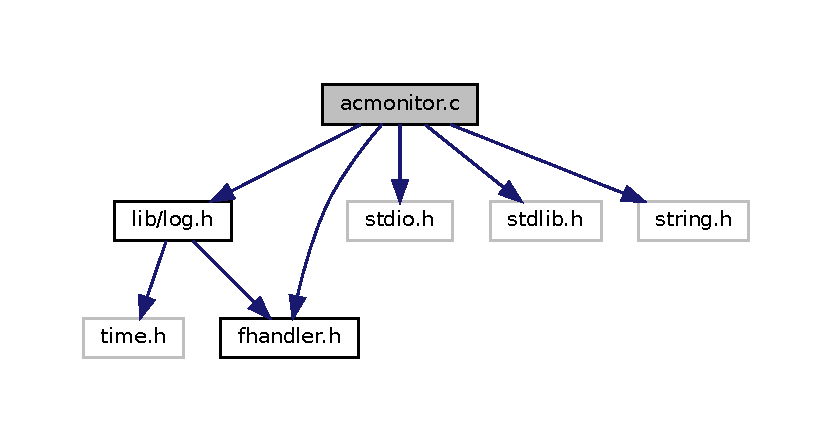
\includegraphics[width=350pt]{acmonitor_8c__incl}
\end{center}
\end{figure}
\subsection*{Data Structures}
\begin{DoxyCompactItemize}
\item 
struct \hyperlink{structlog__entry__text__hash}{log\+\_\+entry\+\_\+text\+\_\+hash}
\end{DoxyCompactItemize}
\subsection*{Macros}
\begin{DoxyCompactItemize}
\item 
\#define \hyperlink{acmonitor_8c_aff6732b7d46ac296a7b8d61ada41d949_aff6732b7d46ac296a7b8d61ada41d949}{\+\_\+\+L\+O\+G\+\_\+\+B\+U\+F\+F\+E\+R\+\_\+\+S\+I\+Z\+E\+\_\+}~1024
\item 
\#define \hyperlink{acmonitor_8c_a73708c27921af699a08573001ea2584d_a73708c27921af699a08573001ea2584d}{\+\_\+\+M\+A\+X\+\_\+\+S\+T\+R\+I\+K\+E\+\_\+}~7
\end{DoxyCompactItemize}
\subsection*{Typedefs}
\begin{DoxyCompactItemize}
\item 
typedef struct \hyperlink{structlog__entry__text__hash}{log\+\_\+entry\+\_\+text\+\_\+hash} \hyperlink{acmonitor_8c_a2c07adb053c6cb67f66231ae9cc7734d_a2c07adb053c6cb67f66231ae9cc7734d}{logf\+\_\+t}
\end{DoxyCompactItemize}
\subsection*{Functions}
\begin{DoxyCompactItemize}
\item 
\hyperlink{acmonitor_8c_a2c07adb053c6cb67f66231ae9cc7734d_a2c07adb053c6cb67f66231ae9cc7734d}{logf\+\_\+t} \hyperlink{acmonitor_8c_a88ee5df83d5ccb61194f75e95db7771b_a88ee5df83d5ccb61194f75e95db7771b}{parse\+\_\+file} (F\+I\+LE $\ast$fp)
\item 
void \hyperlink{acmonitor_8c_a6f1ac7ad36d068e54e8c4b9b03981960_a6f1ac7ad36d068e54e8c4b9b03981960}{print\+\_\+logf} (\hyperlink{acmonitor_8c_a2c07adb053c6cb67f66231ae9cc7734d_a2c07adb053c6cb67f66231ae9cc7734d}{logf\+\_\+t} log)
\item 
int \hyperlink{acmonitor_8c_a0ddf1224851353fc92bfbff6f499fa97_a0ddf1224851353fc92bfbff6f499fa97}{main} (int argc, char $\ast$argv\mbox{[}$\,$\mbox{]})
\end{DoxyCompactItemize}


\subsection{Macro Definition Documentation}
\mbox{\Hypertarget{acmonitor_8c_aff6732b7d46ac296a7b8d61ada41d949_aff6732b7d46ac296a7b8d61ada41d949}\label{acmonitor_8c_aff6732b7d46ac296a7b8d61ada41d949_aff6732b7d46ac296a7b8d61ada41d949}} 
\index{acmonitor.\+c@{acmonitor.\+c}!\+\_\+\+L\+O\+G\+\_\+\+B\+U\+F\+F\+E\+R\+\_\+\+S\+I\+Z\+E\+\_\+@{\+\_\+\+L\+O\+G\+\_\+\+B\+U\+F\+F\+E\+R\+\_\+\+S\+I\+Z\+E\+\_\+}}
\index{\+\_\+\+L\+O\+G\+\_\+\+B\+U\+F\+F\+E\+R\+\_\+\+S\+I\+Z\+E\+\_\+@{\+\_\+\+L\+O\+G\+\_\+\+B\+U\+F\+F\+E\+R\+\_\+\+S\+I\+Z\+E\+\_\+}!acmonitor.\+c@{acmonitor.\+c}}
\subsubsection{\texorpdfstring{\+\_\+\+L\+O\+G\+\_\+\+B\+U\+F\+F\+E\+R\+\_\+\+S\+I\+Z\+E\+\_\+}{\_LOG\_BUFFER\_SIZE\_}}
{\footnotesize\ttfamily \#define \+\_\+\+L\+O\+G\+\_\+\+B\+U\+F\+F\+E\+R\+\_\+\+S\+I\+Z\+E\+\_\+~1024}

\mbox{\Hypertarget{acmonitor_8c_a73708c27921af699a08573001ea2584d_a73708c27921af699a08573001ea2584d}\label{acmonitor_8c_a73708c27921af699a08573001ea2584d_a73708c27921af699a08573001ea2584d}} 
\index{acmonitor.\+c@{acmonitor.\+c}!\+\_\+\+M\+A\+X\+\_\+\+S\+T\+R\+I\+K\+E\+\_\+@{\+\_\+\+M\+A\+X\+\_\+\+S\+T\+R\+I\+K\+E\+\_\+}}
\index{\+\_\+\+M\+A\+X\+\_\+\+S\+T\+R\+I\+K\+E\+\_\+@{\+\_\+\+M\+A\+X\+\_\+\+S\+T\+R\+I\+K\+E\+\_\+}!acmonitor.\+c@{acmonitor.\+c}}
\subsubsection{\texorpdfstring{\+\_\+\+M\+A\+X\+\_\+\+S\+T\+R\+I\+K\+E\+\_\+}{\_MAX\_STRIKE\_}}
{\footnotesize\ttfamily \#define \+\_\+\+M\+A\+X\+\_\+\+S\+T\+R\+I\+K\+E\+\_\+~7}



\subsection{Typedef Documentation}
\mbox{\Hypertarget{acmonitor_8c_a2c07adb053c6cb67f66231ae9cc7734d_a2c07adb053c6cb67f66231ae9cc7734d}\label{acmonitor_8c_a2c07adb053c6cb67f66231ae9cc7734d_a2c07adb053c6cb67f66231ae9cc7734d}} 
\index{acmonitor.\+c@{acmonitor.\+c}!logf\+\_\+t@{logf\+\_\+t}}
\index{logf\+\_\+t@{logf\+\_\+t}!acmonitor.\+c@{acmonitor.\+c}}
\subsubsection{\texorpdfstring{logf\+\_\+t}{logf\_t}}
{\footnotesize\ttfamily typedef struct \hyperlink{structlog__entry__text__hash}{log\+\_\+entry\+\_\+text\+\_\+hash}  \hyperlink{acmonitor_8c_a2c07adb053c6cb67f66231ae9cc7734d_a2c07adb053c6cb67f66231ae9cc7734d}{logf\+\_\+t}}



\subsection{Function Documentation}
\mbox{\Hypertarget{acmonitor_8c_a0ddf1224851353fc92bfbff6f499fa97_a0ddf1224851353fc92bfbff6f499fa97}\label{acmonitor_8c_a0ddf1224851353fc92bfbff6f499fa97_a0ddf1224851353fc92bfbff6f499fa97}} 
\index{acmonitor.\+c@{acmonitor.\+c}!main@{main}}
\index{main@{main}!acmonitor.\+c@{acmonitor.\+c}}
\subsubsection{\texorpdfstring{main()}{main()}}
{\footnotesize\ttfamily int main (\begin{DoxyParamCaption}\item[{int}]{argc,  }\item[{char $\ast$}]{argv\mbox{[}$\,$\mbox{]} }\end{DoxyParamCaption})}

\mbox{\Hypertarget{acmonitor_8c_a88ee5df83d5ccb61194f75e95db7771b_a88ee5df83d5ccb61194f75e95db7771b}\label{acmonitor_8c_a88ee5df83d5ccb61194f75e95db7771b_a88ee5df83d5ccb61194f75e95db7771b}} 
\index{acmonitor.\+c@{acmonitor.\+c}!parse\+\_\+file@{parse\+\_\+file}}
\index{parse\+\_\+file@{parse\+\_\+file}!acmonitor.\+c@{acmonitor.\+c}}
\subsubsection{\texorpdfstring{parse\+\_\+file()}{parse\_file()}}
{\footnotesize\ttfamily \hyperlink{acmonitor_8c_a2c07adb053c6cb67f66231ae9cc7734d_a2c07adb053c6cb67f66231ae9cc7734d}{logf\+\_\+t} parse\+\_\+file (\begin{DoxyParamCaption}\item[{F\+I\+LE $\ast$}]{fp }\end{DoxyParamCaption})}

\mbox{\Hypertarget{acmonitor_8c_a6f1ac7ad36d068e54e8c4b9b03981960_a6f1ac7ad36d068e54e8c4b9b03981960}\label{acmonitor_8c_a6f1ac7ad36d068e54e8c4b9b03981960_a6f1ac7ad36d068e54e8c4b9b03981960}} 
\index{acmonitor.\+c@{acmonitor.\+c}!print\+\_\+logf@{print\+\_\+logf}}
\index{print\+\_\+logf@{print\+\_\+logf}!acmonitor.\+c@{acmonitor.\+c}}
\subsubsection{\texorpdfstring{print\+\_\+logf()}{print\_logf()}}
{\footnotesize\ttfamily void print\+\_\+logf (\begin{DoxyParamCaption}\item[{\hyperlink{acmonitor_8c_a2c07adb053c6cb67f66231ae9cc7734d_a2c07adb053c6cb67f66231ae9cc7734d}{logf\+\_\+t}}]{log }\end{DoxyParamCaption})}


\hypertarget{fhandler_8c}{}\section{fhandler.\+c File Reference}
\label{fhandler_8c}\index{fhandler.\+c@{fhandler.\+c}}
{\ttfamily \#include \char`\"{}fhandler.\+h\char`\"{}}\newline
{\ttfamily \#include $<$stdio.\+h$>$}\newline
{\ttfamily \#include $<$stdlib.\+h$>$}\newline
{\ttfamily \#include $<$dlfcn.\+h$>$}\newline
Include dependency graph for fhandler.\+c\+:\nopagebreak
\begin{figure}[H]
\begin{center}
\leavevmode
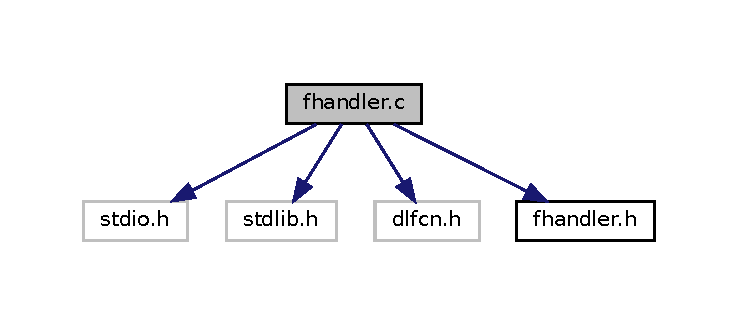
\includegraphics[width=350pt]{fhandler_8c__incl}
\end{center}
\end{figure}
\subsection*{Functions}
\begin{DoxyCompactItemize}
\item 
void \hyperlink{fhandler_8c_a9b1ada6e94cd79a619e282d13b8529d7_a9b1ada6e94cd79a619e282d13b8529d7}{Handle} (const char $\ast$\+\_\+\+\_\+lib, const char $\ast$\+\_\+\+\_\+func, void $\ast$\+\_\+funcp)
\begin{DoxyCompactList}\small\item\em Handles the dynamic linking of the functions. \end{DoxyCompactList}\end{DoxyCompactItemize}


\subsection{Function Documentation}
\mbox{\Hypertarget{fhandler_8c_a9b1ada6e94cd79a619e282d13b8529d7_a9b1ada6e94cd79a619e282d13b8529d7}\label{fhandler_8c_a9b1ada6e94cd79a619e282d13b8529d7_a9b1ada6e94cd79a619e282d13b8529d7}} 
\index{fhandler.\+c@{fhandler.\+c}!Handle@{Handle}}
\index{Handle@{Handle}!fhandler.\+c@{fhandler.\+c}}
\subsubsection{\texorpdfstring{Handle()}{Handle()}}
{\footnotesize\ttfamily void Handle (\begin{DoxyParamCaption}\item[{const char $\ast$}]{\+\_\+\+\_\+lib,  }\item[{const char $\ast$}]{\+\_\+\+\_\+func,  }\item[{void $\ast$}]{\+\_\+funcp }\end{DoxyParamCaption})}



Handles the dynamic linking of the functions. 


\begin{DoxyParams}{Parameters}
{\em \+\_\+\+\_\+lib} & The library name to be linked. \\
\hline
{\em \+\_\+\+\_\+func} & The function name to be linked. \\
\hline
{\em \+\_\+funcp} & The pointer to the function to be linked. \\
\hline
\end{DoxyParams}

\hypertarget{fhandler_8h}{}\section{fhandler.\+h File Reference}
\label{fhandler_8h}\index{fhandler.\+h@{fhandler.\+h}}
This graph shows which files directly or indirectly include this file\+:\nopagebreak
\begin{figure}[H]
\begin{center}
\leavevmode
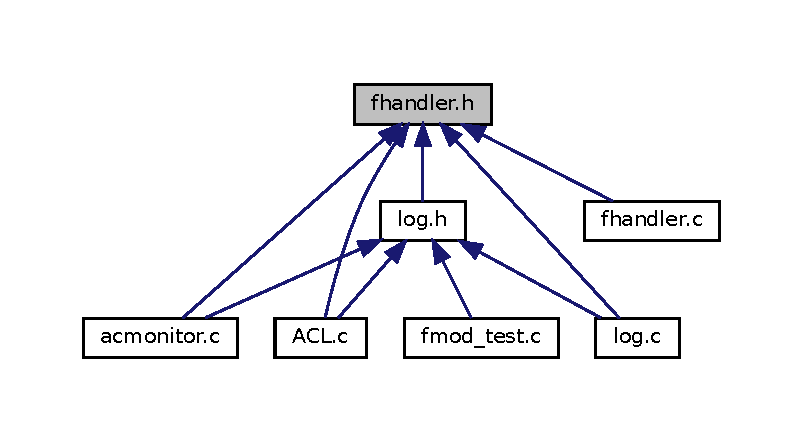
\includegraphics[width=350pt]{fhandler_8h__dep__incl}
\end{center}
\end{figure}
\subsection*{Macros}
\begin{DoxyCompactItemize}
\item 
\#define \hyperlink{fhandler_8h_a369266c24eacffb87046522897a570d5_a369266c24eacffb87046522897a570d5}{\+\_\+\+G\+N\+U\+\_\+\+S\+O\+U\+R\+CE}
\end{DoxyCompactItemize}
\subsection*{Functions}
\begin{DoxyCompactItemize}
\item 
void \hyperlink{fhandler_8h_a9b1ada6e94cd79a619e282d13b8529d7_a9b1ada6e94cd79a619e282d13b8529d7}{Handle} (const char $\ast$\+\_\+\+\_\+lib, const char $\ast$\+\_\+\+\_\+func, void $\ast$\+\_\+funcp)
\begin{DoxyCompactList}\small\item\em Handles the dynamic linking of the functions. \end{DoxyCompactList}\end{DoxyCompactItemize}


\subsection{Macro Definition Documentation}
\mbox{\Hypertarget{fhandler_8h_a369266c24eacffb87046522897a570d5_a369266c24eacffb87046522897a570d5}\label{fhandler_8h_a369266c24eacffb87046522897a570d5_a369266c24eacffb87046522897a570d5}} 
\index{fhandler.\+h@{fhandler.\+h}!\+\_\+\+G\+N\+U\+\_\+\+S\+O\+U\+R\+CE@{\+\_\+\+G\+N\+U\+\_\+\+S\+O\+U\+R\+CE}}
\index{\+\_\+\+G\+N\+U\+\_\+\+S\+O\+U\+R\+CE@{\+\_\+\+G\+N\+U\+\_\+\+S\+O\+U\+R\+CE}!fhandler.\+h@{fhandler.\+h}}
\subsubsection{\texorpdfstring{\+\_\+\+G\+N\+U\+\_\+\+S\+O\+U\+R\+CE}{\_GNU\_SOURCE}}
{\footnotesize\ttfamily \#define \+\_\+\+G\+N\+U\+\_\+\+S\+O\+U\+R\+CE}



\subsection{Function Documentation}
\mbox{\Hypertarget{fhandler_8h_a9b1ada6e94cd79a619e282d13b8529d7_a9b1ada6e94cd79a619e282d13b8529d7}\label{fhandler_8h_a9b1ada6e94cd79a619e282d13b8529d7_a9b1ada6e94cd79a619e282d13b8529d7}} 
\index{fhandler.\+h@{fhandler.\+h}!Handle@{Handle}}
\index{Handle@{Handle}!fhandler.\+h@{fhandler.\+h}}
\subsubsection{\texorpdfstring{Handle()}{Handle()}}
{\footnotesize\ttfamily void Handle (\begin{DoxyParamCaption}\item[{const char $\ast$}]{\+\_\+\+\_\+lib,  }\item[{const char $\ast$}]{\+\_\+\+\_\+func,  }\item[{void $\ast$}]{\+\_\+funcp }\end{DoxyParamCaption})}



Handles the dynamic linking of the functions. 


\begin{DoxyParams}{Parameters}
{\em \+\_\+\+\_\+lib} & The library name to be linked. \\
\hline
{\em \+\_\+\+\_\+func} & The function name to be linked. \\
\hline
{\em \+\_\+funcp} & The pointer to the function to be linked. \\
\hline
\end{DoxyParams}

\hypertarget{fperm__test_8c}{}\section{fperm\+\_\+test.\+c File Reference}
\label{fperm__test_8c}\index{fperm\+\_\+test.\+c@{fperm\+\_\+test.\+c}}
{\ttfamily \#include $<$sys/types.\+h$>$}\newline
{\ttfamily \#include $<$sys/stat.\+h$>$}\newline
{\ttfamily \#include $<$unistd.\+h$>$}\newline
{\ttfamily \#include $<$stdio.\+h$>$}\newline
{\ttfamily \#include $<$grp.\+h$>$}\newline
{\ttfamily \#include $<$pwd.\+h$>$}\newline
{\ttfamily \#include $<$errno.\+h$>$}\newline
{\ttfamily \#include $<$stdlib.\+h$>$}\newline
{\ttfamily \#include $<$string.\+h$>$}\newline
Include dependency graph for fperm\+\_\+test.\+c\+:\nopagebreak
\begin{figure}[H]
\begin{center}
\leavevmode
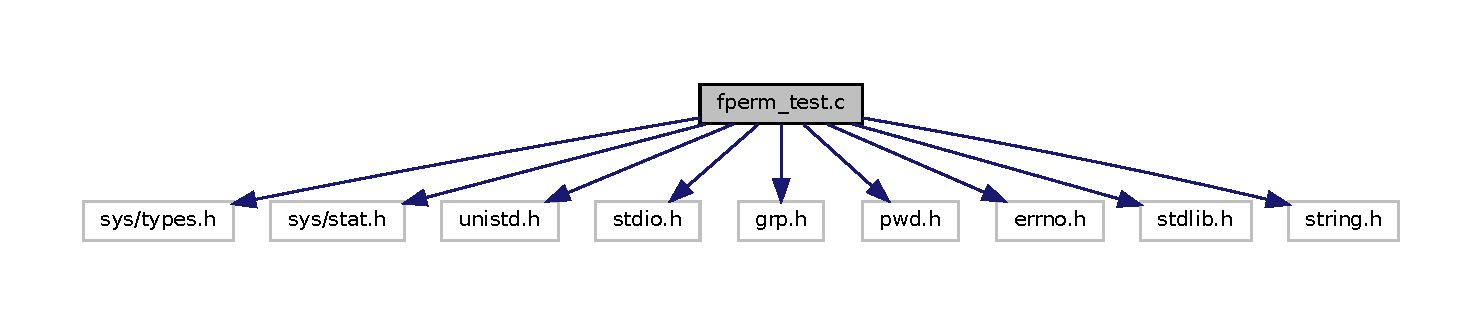
\includegraphics[width=350pt]{fperm__test_8c__incl}
\end{center}
\end{figure}
\subsection*{Macros}
\begin{DoxyCompactItemize}
\item 
\#define \hyperlink{fperm__test_8c_a8d23feea868a983c8c2b661e1e16972f_a8d23feea868a983c8c2b661e1e16972f}{R\+ED}~\char`\"{}\textbackslash{}x1B\mbox{[}31m\char`\"{}
\item 
\#define \hyperlink{fperm__test_8c_aea69ffbacdcdf16c21b8c9961df84448_aea69ffbacdcdf16c21b8c9961df84448}{G\+RN}~\char`\"{}\textbackslash{}x1B\mbox{[}32m\char`\"{}
\item 
\#define \hyperlink{fperm__test_8c_a96fac03c4ab3363f06a0328e0e53a40c_a96fac03c4ab3363f06a0328e0e53a40c}{Y\+EL}~\char`\"{}\textbackslash{}x1B\mbox{[}33m\char`\"{}
\item 
\#define \hyperlink{fperm__test_8c_add9307de87f38e77d336751e305886f6_add9307de87f38e77d336751e305886f6}{B\+LU}~\char`\"{}\textbackslash{}x1B\mbox{[}34m\char`\"{}
\item 
\#define \hyperlink{fperm__test_8c_af54a5a977c0c499323d656315f008ee0_af54a5a977c0c499323d656315f008ee0}{M\+AG}~\char`\"{}\textbackslash{}x1B\mbox{[}35m\char`\"{}
\item 
\#define \hyperlink{fperm__test_8c_adc708fa688f5d78db361f66c36f0f807_adc708fa688f5d78db361f66c36f0f807}{C\+YN}~\char`\"{}\textbackslash{}x1B\mbox{[}36m\char`\"{}
\item 
\#define \hyperlink{fperm__test_8c_aeaf3a04d5bf63b204689a714718ea930_aeaf3a04d5bf63b204689a714718ea930}{W\+HT}~\char`\"{}\textbackslash{}x1B\mbox{[}37m\char`\"{}
\item 
\#define \hyperlink{fperm__test_8c_ab702106cf3b3e96750b6845ded4e0299_ab702106cf3b3e96750b6845ded4e0299}{R\+E\+S\+ET}~\char`\"{}\textbackslash{}x1B\mbox{[}0m\char`\"{}
\end{DoxyCompactItemize}
\subsection*{Functions}
\begin{DoxyCompactItemize}
\item 
int \hyperlink{fperm__test_8c_a711d0bb2170aecd6cda15f498aa8660f_a711d0bb2170aecd6cda15f498aa8660f}{test\+Write} ()
\item 
int \hyperlink{fperm__test_8c_a82c9fc590374ae3e8a847687266c8537_a82c9fc590374ae3e8a847687266c8537}{test\+Read} ()
\item 
int \hyperlink{fperm__test_8c_a4c730ced6041a87cf27be08a5cc591af_a4c730ced6041a87cf27be08a5cc591af}{test\+Exec} ()
\item 
int \hyperlink{fperm__test_8c_ae66f6b31b5ad750f1fe042a706a4e3d4_ae66f6b31b5ad750f1fe042a706a4e3d4}{main} ()
\end{DoxyCompactItemize}
\subsection*{Variables}
\begin{DoxyCompactItemize}
\item 
char \hyperlink{fperm__test_8c_a9acefa3eb5b801834cb9b7a7453b41e0_a9acefa3eb5b801834cb9b7a7453b41e0}{paths} \mbox{[}$\,$\mbox{]}\mbox{[}256\mbox{]}
\end{DoxyCompactItemize}


\subsection{Macro Definition Documentation}
\mbox{\Hypertarget{fperm__test_8c_add9307de87f38e77d336751e305886f6_add9307de87f38e77d336751e305886f6}\label{fperm__test_8c_add9307de87f38e77d336751e305886f6_add9307de87f38e77d336751e305886f6}} 
\index{fperm\+\_\+test.\+c@{fperm\+\_\+test.\+c}!B\+LU@{B\+LU}}
\index{B\+LU@{B\+LU}!fperm\+\_\+test.\+c@{fperm\+\_\+test.\+c}}
\subsubsection{\texorpdfstring{B\+LU}{BLU}}
{\footnotesize\ttfamily \#define B\+LU~\char`\"{}\textbackslash{}x1B\mbox{[}34m\char`\"{}}

\mbox{\Hypertarget{fperm__test_8c_adc708fa688f5d78db361f66c36f0f807_adc708fa688f5d78db361f66c36f0f807}\label{fperm__test_8c_adc708fa688f5d78db361f66c36f0f807_adc708fa688f5d78db361f66c36f0f807}} 
\index{fperm\+\_\+test.\+c@{fperm\+\_\+test.\+c}!C\+YN@{C\+YN}}
\index{C\+YN@{C\+YN}!fperm\+\_\+test.\+c@{fperm\+\_\+test.\+c}}
\subsubsection{\texorpdfstring{C\+YN}{CYN}}
{\footnotesize\ttfamily \#define C\+YN~\char`\"{}\textbackslash{}x1B\mbox{[}36m\char`\"{}}

\mbox{\Hypertarget{fperm__test_8c_aea69ffbacdcdf16c21b8c9961df84448_aea69ffbacdcdf16c21b8c9961df84448}\label{fperm__test_8c_aea69ffbacdcdf16c21b8c9961df84448_aea69ffbacdcdf16c21b8c9961df84448}} 
\index{fperm\+\_\+test.\+c@{fperm\+\_\+test.\+c}!G\+RN@{G\+RN}}
\index{G\+RN@{G\+RN}!fperm\+\_\+test.\+c@{fperm\+\_\+test.\+c}}
\subsubsection{\texorpdfstring{G\+RN}{GRN}}
{\footnotesize\ttfamily \#define G\+RN~\char`\"{}\textbackslash{}x1B\mbox{[}32m\char`\"{}}

\mbox{\Hypertarget{fperm__test_8c_af54a5a977c0c499323d656315f008ee0_af54a5a977c0c499323d656315f008ee0}\label{fperm__test_8c_af54a5a977c0c499323d656315f008ee0_af54a5a977c0c499323d656315f008ee0}} 
\index{fperm\+\_\+test.\+c@{fperm\+\_\+test.\+c}!M\+AG@{M\+AG}}
\index{M\+AG@{M\+AG}!fperm\+\_\+test.\+c@{fperm\+\_\+test.\+c}}
\subsubsection{\texorpdfstring{M\+AG}{MAG}}
{\footnotesize\ttfamily \#define M\+AG~\char`\"{}\textbackslash{}x1B\mbox{[}35m\char`\"{}}

\mbox{\Hypertarget{fperm__test_8c_a8d23feea868a983c8c2b661e1e16972f_a8d23feea868a983c8c2b661e1e16972f}\label{fperm__test_8c_a8d23feea868a983c8c2b661e1e16972f_a8d23feea868a983c8c2b661e1e16972f}} 
\index{fperm\+\_\+test.\+c@{fperm\+\_\+test.\+c}!R\+ED@{R\+ED}}
\index{R\+ED@{R\+ED}!fperm\+\_\+test.\+c@{fperm\+\_\+test.\+c}}
\subsubsection{\texorpdfstring{R\+ED}{RED}}
{\footnotesize\ttfamily \#define R\+ED~\char`\"{}\textbackslash{}x1B\mbox{[}31m\char`\"{}}

\mbox{\Hypertarget{fperm__test_8c_ab702106cf3b3e96750b6845ded4e0299_ab702106cf3b3e96750b6845ded4e0299}\label{fperm__test_8c_ab702106cf3b3e96750b6845ded4e0299_ab702106cf3b3e96750b6845ded4e0299}} 
\index{fperm\+\_\+test.\+c@{fperm\+\_\+test.\+c}!R\+E\+S\+ET@{R\+E\+S\+ET}}
\index{R\+E\+S\+ET@{R\+E\+S\+ET}!fperm\+\_\+test.\+c@{fperm\+\_\+test.\+c}}
\subsubsection{\texorpdfstring{R\+E\+S\+ET}{RESET}}
{\footnotesize\ttfamily \#define R\+E\+S\+ET~\char`\"{}\textbackslash{}x1B\mbox{[}0m\char`\"{}}

\mbox{\Hypertarget{fperm__test_8c_aeaf3a04d5bf63b204689a714718ea930_aeaf3a04d5bf63b204689a714718ea930}\label{fperm__test_8c_aeaf3a04d5bf63b204689a714718ea930_aeaf3a04d5bf63b204689a714718ea930}} 
\index{fperm\+\_\+test.\+c@{fperm\+\_\+test.\+c}!W\+HT@{W\+HT}}
\index{W\+HT@{W\+HT}!fperm\+\_\+test.\+c@{fperm\+\_\+test.\+c}}
\subsubsection{\texorpdfstring{W\+HT}{WHT}}
{\footnotesize\ttfamily \#define W\+HT~\char`\"{}\textbackslash{}x1B\mbox{[}37m\char`\"{}}

\mbox{\Hypertarget{fperm__test_8c_a96fac03c4ab3363f06a0328e0e53a40c_a96fac03c4ab3363f06a0328e0e53a40c}\label{fperm__test_8c_a96fac03c4ab3363f06a0328e0e53a40c_a96fac03c4ab3363f06a0328e0e53a40c}} 
\index{fperm\+\_\+test.\+c@{fperm\+\_\+test.\+c}!Y\+EL@{Y\+EL}}
\index{Y\+EL@{Y\+EL}!fperm\+\_\+test.\+c@{fperm\+\_\+test.\+c}}
\subsubsection{\texorpdfstring{Y\+EL}{YEL}}
{\footnotesize\ttfamily \#define Y\+EL~\char`\"{}\textbackslash{}x1B\mbox{[}33m\char`\"{}}



\subsection{Function Documentation}
\mbox{\Hypertarget{fperm__test_8c_ae66f6b31b5ad750f1fe042a706a4e3d4_ae66f6b31b5ad750f1fe042a706a4e3d4}\label{fperm__test_8c_ae66f6b31b5ad750f1fe042a706a4e3d4_ae66f6b31b5ad750f1fe042a706a4e3d4}} 
\index{fperm\+\_\+test.\+c@{fperm\+\_\+test.\+c}!main@{main}}
\index{main@{main}!fperm\+\_\+test.\+c@{fperm\+\_\+test.\+c}}
\subsubsection{\texorpdfstring{main()}{main()}}
{\footnotesize\ttfamily int main (\begin{DoxyParamCaption}\item[{void}]{ }\end{DoxyParamCaption})}

\mbox{\Hypertarget{fperm__test_8c_a4c730ced6041a87cf27be08a5cc591af_a4c730ced6041a87cf27be08a5cc591af}\label{fperm__test_8c_a4c730ced6041a87cf27be08a5cc591af_a4c730ced6041a87cf27be08a5cc591af}} 
\index{fperm\+\_\+test.\+c@{fperm\+\_\+test.\+c}!test\+Exec@{test\+Exec}}
\index{test\+Exec@{test\+Exec}!fperm\+\_\+test.\+c@{fperm\+\_\+test.\+c}}
\subsubsection{\texorpdfstring{test\+Exec()}{testExec()}}
{\footnotesize\ttfamily int test\+Exec (\begin{DoxyParamCaption}{ }\end{DoxyParamCaption})}

\mbox{\Hypertarget{fperm__test_8c_a82c9fc590374ae3e8a847687266c8537_a82c9fc590374ae3e8a847687266c8537}\label{fperm__test_8c_a82c9fc590374ae3e8a847687266c8537_a82c9fc590374ae3e8a847687266c8537}} 
\index{fperm\+\_\+test.\+c@{fperm\+\_\+test.\+c}!test\+Read@{test\+Read}}
\index{test\+Read@{test\+Read}!fperm\+\_\+test.\+c@{fperm\+\_\+test.\+c}}
\subsubsection{\texorpdfstring{test\+Read()}{testRead()}}
{\footnotesize\ttfamily int test\+Read (\begin{DoxyParamCaption}{ }\end{DoxyParamCaption})}

\mbox{\Hypertarget{fperm__test_8c_a711d0bb2170aecd6cda15f498aa8660f_a711d0bb2170aecd6cda15f498aa8660f}\label{fperm__test_8c_a711d0bb2170aecd6cda15f498aa8660f_a711d0bb2170aecd6cda15f498aa8660f}} 
\index{fperm\+\_\+test.\+c@{fperm\+\_\+test.\+c}!test\+Write@{test\+Write}}
\index{test\+Write@{test\+Write}!fperm\+\_\+test.\+c@{fperm\+\_\+test.\+c}}
\subsubsection{\texorpdfstring{test\+Write()}{testWrite()}}
{\footnotesize\ttfamily int test\+Write (\begin{DoxyParamCaption}{ }\end{DoxyParamCaption})}

In this test we check whether our program can bypass permissions.

We have created 18 files with different permissions and we try to read, write and execute them. 

\subsection{Variable Documentation}
\mbox{\Hypertarget{fperm__test_8c_a9acefa3eb5b801834cb9b7a7453b41e0_a9acefa3eb5b801834cb9b7a7453b41e0}\label{fperm__test_8c_a9acefa3eb5b801834cb9b7a7453b41e0_a9acefa3eb5b801834cb9b7a7453b41e0}} 
\index{fperm\+\_\+test.\+c@{fperm\+\_\+test.\+c}!paths@{paths}}
\index{paths@{paths}!fperm\+\_\+test.\+c@{fperm\+\_\+test.\+c}}
\subsubsection{\texorpdfstring{paths}{paths}}
{\footnotesize\ttfamily char paths\mbox{[}$\,$\mbox{]}\mbox{[}256\mbox{]}}

{\bfseries Initial value\+:}
\begin{DoxyCode}
= \{
    \textcolor{stringliteral}{"test/.testfiles/user\_read.c"},
    \textcolor{stringliteral}{"test/.testfiles/group\_read.c"},
    \textcolor{stringliteral}{"test/.testfiles/other\_read.c"},
    \textcolor{stringliteral}{"test/.testfiles/user\_write.c"},
    \textcolor{stringliteral}{"test/.testfiles/group\_write.c"},
    \textcolor{stringliteral}{"test/.testfiles/other\_write.c"},
    \textcolor{stringliteral}{"test/.testfiles/user\_execute"},
    \textcolor{stringliteral}{"test/.testfiles/group\_execute"},
    \textcolor{stringliteral}{"test/.testfiles/other\_execute"},
    \textcolor{stringliteral}{"test/.testfiles/user\_read\_write.c"},
    \textcolor{stringliteral}{"test/.testfiles/group\_read\_write.c"},
    \textcolor{stringliteral}{"test/.testfiles/other\_read\_write.c"},
    \textcolor{stringliteral}{"test/.testfiles/user\_read\_execute"},
    \textcolor{stringliteral}{"test/.testfiles/group\_read\_execute"},
    \textcolor{stringliteral}{"test/.testfiles/other\_read\_execute"},
    \textcolor{stringliteral}{"test/.testfiles/user\_write\_execute"},
    \textcolor{stringliteral}{"test/.testfiles/group\_write\_execute"},
    \textcolor{stringliteral}{"test/.testfiles/other\_write\_execute"}
\}
\end{DoxyCode}

\hypertarget{log_8c}{}\section{log.\+c File Reference}
\label{log_8c}\index{log.\+c@{log.\+c}}
{\ttfamily \#include \char`\"{}log.\+h\char`\"{}}\newline
{\ttfamily \#include $<$stdio.\+h$>$}\newline
{\ttfamily \#include $<$stdlib.\+h$>$}\newline
{\ttfamily \#include $<$string.\+h$>$}\newline
{\ttfamily \#include $<$dlfcn.\+h$>$}\newline
{\ttfamily \#include $<$time.\+h$>$}\newline
{\ttfamily \#include $<$unistd.\+h$>$}\newline
{\ttfamily \#include $<$stdarg.\+h$>$}\newline
{\ttfamily \#include \char`\"{}fhandler.\+h\char`\"{}}\newline
Include dependency graph for log.\+c\+:
\nopagebreak
\begin{figure}[H]
\begin{center}
\leavevmode
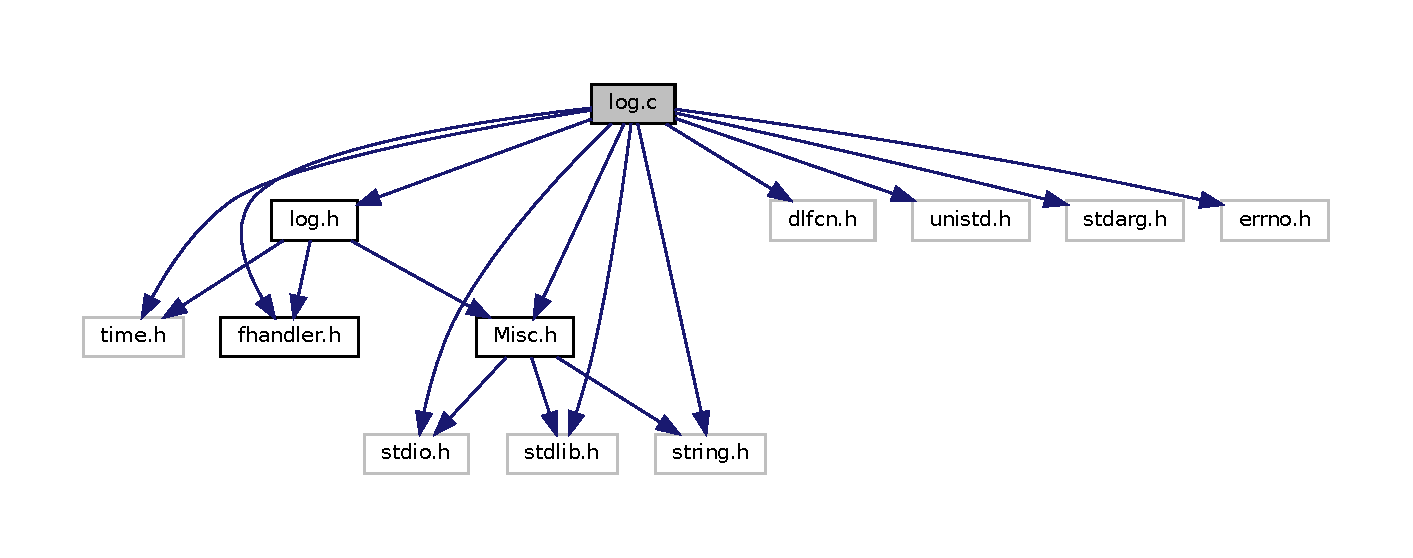
\includegraphics[width=350pt]{log_8c__incl}
\end{center}
\end{figure}
\subsection*{Functions}
\begin{DoxyCompactItemize}
\item 
struct tm \hyperlink{log_8c_a2de5fe84ca15039e1b007634ccef1651_a2de5fe84ca15039e1b007634ccef1651}{date\+\_\+and\+\_\+time} ()
\begin{DoxyCompactList}\small\item\em Create a timestamp object with the current date and time. \end{DoxyCompactList}\item 
void \hyperlink{log_8c_ab3a7d9a8e25e365afb72e557f60ba45f_ab3a7d9a8e25e365afb72e557f60ba45f}{print\+\_\+log\+\_\+to\+\_\+file} (\hyperlink{log_8h_abd600feddcc5ca71fa3f3afa84eee569_abd600feddcc5ca71fa3f3afa84eee569}{log\+\_\+t} \hyperlink{structlog__entry}{log\+\_\+entry})
\begin{DoxyCompactList}\small\item\em Prints the log entry to the log file. \end{DoxyCompactList}\item 
\hyperlink{log_8h_abd600feddcc5ca71fa3f3afa84eee569_abd600feddcc5ca71fa3f3afa84eee569}{log\+\_\+t} \hyperlink{log_8c_a208f5ebd87e3ff13ab84ab2d57c46974_a208f5ebd87e3ff13ab84ab2d57c46974}{create\+\_\+log} (const char $\ast$path, const \hyperlink{log_8h_ab20c54dfb1eb1323b9a3cfe2e6a76270_ab20c54dfb1eb1323b9a3cfe2e6a76270}{access\+\_\+t} access, const int action\+\_\+denied, unsigned char fingerprint\mbox{[}16\mbox{]})
\begin{DoxyCompactList}\small\item\em Creates a log entry. \end{DoxyCompactList}\end{DoxyCompactItemize}


\subsection{Function Documentation}
\mbox{\Hypertarget{log_8c_a208f5ebd87e3ff13ab84ab2d57c46974_a208f5ebd87e3ff13ab84ab2d57c46974}\label{log_8c_a208f5ebd87e3ff13ab84ab2d57c46974_a208f5ebd87e3ff13ab84ab2d57c46974}} 
\index{log.\+c@{log.\+c}!create\+\_\+log@{create\+\_\+log}}
\index{create\+\_\+log@{create\+\_\+log}!log.\+c@{log.\+c}}
\subsubsection{\texorpdfstring{create\+\_\+log()}{create\_log()}}
{\footnotesize\ttfamily \hyperlink{log_8h_abd600feddcc5ca71fa3f3afa84eee569_abd600feddcc5ca71fa3f3afa84eee569}{log\+\_\+t} create\+\_\+log (\begin{DoxyParamCaption}\item[{const char $\ast$}]{path,  }\item[{const \hyperlink{log_8h_ab20c54dfb1eb1323b9a3cfe2e6a76270_ab20c54dfb1eb1323b9a3cfe2e6a76270}{access\+\_\+t}}]{access,  }\item[{const int}]{action\+\_\+denied,  }\item[{unsigned char}]{fingerprint\mbox{[}16\mbox{]} }\end{DoxyParamCaption})}



Creates a log entry. 


\begin{DoxyParams}{Parameters}
{\em path} & The absolute path of the file. \\
\hline
{\em access} & The access type. see access\+\_\+t \\
\hline
{\em action\+\_\+denied} & 1 if the action was denied, else 0. \\
\hline
{\em fingerprint} & The fingerprint of the file. \\
\hline
\end{DoxyParams}
\mbox{\Hypertarget{log_8c_a2de5fe84ca15039e1b007634ccef1651_a2de5fe84ca15039e1b007634ccef1651}\label{log_8c_a2de5fe84ca15039e1b007634ccef1651_a2de5fe84ca15039e1b007634ccef1651}} 
\index{log.\+c@{log.\+c}!date\+\_\+and\+\_\+time@{date\+\_\+and\+\_\+time}}
\index{date\+\_\+and\+\_\+time@{date\+\_\+and\+\_\+time}!log.\+c@{log.\+c}}
\subsubsection{\texorpdfstring{date\+\_\+and\+\_\+time()}{date\_and\_time()}}
{\footnotesize\ttfamily struct tm date\+\_\+and\+\_\+time (\begin{DoxyParamCaption}{ }\end{DoxyParamCaption})}



Create a timestamp object with the current date and time. 

\begin{DoxyReturn}{Returns}
struct tm The current date and time. 
\end{DoxyReturn}
\mbox{\Hypertarget{log_8c_ab3a7d9a8e25e365afb72e557f60ba45f_ab3a7d9a8e25e365afb72e557f60ba45f}\label{log_8c_ab3a7d9a8e25e365afb72e557f60ba45f_ab3a7d9a8e25e365afb72e557f60ba45f}} 
\index{log.\+c@{log.\+c}!print\+\_\+log\+\_\+to\+\_\+file@{print\+\_\+log\+\_\+to\+\_\+file}}
\index{print\+\_\+log\+\_\+to\+\_\+file@{print\+\_\+log\+\_\+to\+\_\+file}!log.\+c@{log.\+c}}
\subsubsection{\texorpdfstring{print\+\_\+log\+\_\+to\+\_\+file()}{print\_log\_to\_file()}}
{\footnotesize\ttfamily void print\+\_\+log\+\_\+to\+\_\+file (\begin{DoxyParamCaption}\item[{\hyperlink{log_8h_abd600feddcc5ca71fa3f3afa84eee569_abd600feddcc5ca71fa3f3afa84eee569}{log\+\_\+t}}]{log\+\_\+entry }\end{DoxyParamCaption})}



Prints the log entry to the log file. 


\begin{DoxyParams}{Parameters}
{\em \hyperlink{structlog__entry}{log\+\_\+entry}} & The log entry to be printed. \\
\hline
\end{DoxyParams}

\hypertarget{log_8h}{}\section{log.\+h File Reference}
\label{log_8h}\index{log.\+h@{log.\+h}}
{\ttfamily \#include $<$time.\+h$>$}\newline
{\ttfamily \#include \char`\"{}fhandler.\+h\char`\"{}}\newline
{\ttfamily \#include \char`\"{}Misc.\+h\char`\"{}}\newline
Include dependency graph for log.\+h\+:\nopagebreak
\begin{figure}[H]
\begin{center}
\leavevmode
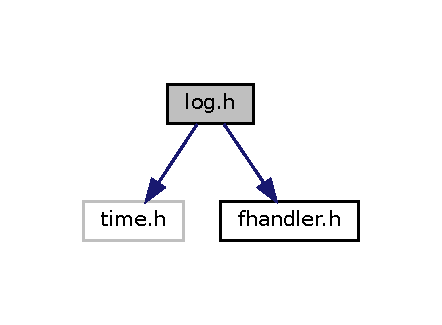
\includegraphics[width=350pt]{log_8h__incl}
\end{center}
\end{figure}
This graph shows which files directly or indirectly include this file\+:\nopagebreak
\begin{figure}[H]
\begin{center}
\leavevmode
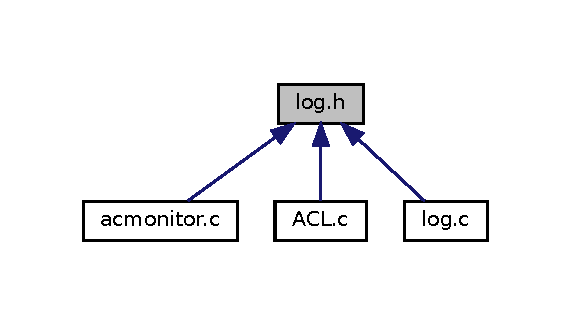
\includegraphics[width=350pt]{log_8h__dep__incl}
\end{center}
\end{figure}
\subsection*{Data Structures}
\begin{DoxyCompactItemize}
\item 
struct \hyperlink{structlog__entry}{log\+\_\+entry}
\begin{DoxyCompactList}\small\item\em The log entry. \end{DoxyCompactList}\item 
struct \hyperlink{structlog__entry__s}{log\+\_\+entry\+\_\+s}
\begin{DoxyCompactList}\small\item\em The log entry in strings format. \end{DoxyCompactList}\item 
struct \hyperlink{structuser__history}{user\+\_\+history}
\begin{DoxyCompactList}\small\item\em User history in the log. Contains all files the user attempted ro access or modify but was rejected. \end{DoxyCompactList}\item 
struct \hyperlink{structfile__history}{file\+\_\+history}
\begin{DoxyCompactList}\small\item\em File history in the log. Contains logs regarding a file. \end{DoxyCompactList}\end{DoxyCompactItemize}
\subsection*{Macros}
\begin{DoxyCompactItemize}
\item 
\#define \hyperlink{log_8h_a286c666b6725cb6f32fbd5500f41dd9f_a286c666b6725cb6f32fbd5500f41dd9f}{\+\_\+\+L\+O\+G\+\_\+\+F\+I\+L\+E\+\_\+\+P\+A\+T\+H\+\_\+}~\char`\"{}etc/log.\+txt\char`\"{}
\begin{DoxyCompactList}\small\item\em Handles all operations regarding the log file. \end{DoxyCompactList}\end{DoxyCompactItemize}
\subsection*{Typedefs}
\begin{DoxyCompactItemize}
\item 
typedef enum \hyperlink{log_8h_a1f5bf9b97a6a0e44df8bdfe6c9779e24_a1f5bf9b97a6a0e44df8bdfe6c9779e24}{access\+\_\+types} \hyperlink{log_8h_ab20c54dfb1eb1323b9a3cfe2e6a76270_ab20c54dfb1eb1323b9a3cfe2e6a76270}{access\+\_\+t}
\begin{DoxyCompactList}\small\item\em The access types. \end{DoxyCompactList}\item 
typedef struct \hyperlink{structlog__entry}{log\+\_\+entry} \hyperlink{log_8h_a9146f9d95d54274f118322bcf7f713ef_a9146f9d95d54274f118322bcf7f713ef}{logf\+\_\+t}
\begin{DoxyCompactList}\small\item\em The log entry. \end{DoxyCompactList}\item 
typedef struct \hyperlink{structlog__entry__s}{log\+\_\+entry\+\_\+s} \hyperlink{log_8h_a6e294c3f610f2a78fe6f6bc8592c7e90_a6e294c3f610f2a78fe6f6bc8592c7e90}{logs\+\_\+t}
\begin{DoxyCompactList}\small\item\em The log entry in strings format. \end{DoxyCompactList}\item 
typedef struct \hyperlink{structuser__history}{user\+\_\+history} \hyperlink{log_8h_adae9bf82e84f8e9ba2b5d82c481fd32a_adae9bf82e84f8e9ba2b5d82c481fd32a}{user\+\_\+history\+\_\+t}
\begin{DoxyCompactList}\small\item\em User history in the log. Contains all files the user attempted ro access or modify but was rejected. \end{DoxyCompactList}\item 
typedef struct \hyperlink{structfile__history}{file\+\_\+history} \hyperlink{log_8h_a5eba967092586c4763c2fbe89d22a634_a5eba967092586c4763c2fbe89d22a634}{file\+\_\+history\+\_\+t}
\begin{DoxyCompactList}\small\item\em File history in the log. Contains logs regarding a file. \end{DoxyCompactList}\end{DoxyCompactItemize}
\subsection*{Enumerations}
\begin{DoxyCompactItemize}
\item 
enum \hyperlink{log_8h_a1f5bf9b97a6a0e44df8bdfe6c9779e24_a1f5bf9b97a6a0e44df8bdfe6c9779e24}{access\+\_\+types} \{ \newline
\hyperlink{log_8h_a1f5bf9b97a6a0e44df8bdfe6c9779e24_a1f5bf9b97a6a0e44df8bdfe6c9779e24acb4c076c6c5acda9b100eda359c1275e}{\+\_\+\+\_\+\+C\+R\+E\+A\+T\+I\+ON}, 
\hyperlink{log_8h_a1f5bf9b97a6a0e44df8bdfe6c9779e24_a1f5bf9b97a6a0e44df8bdfe6c9779e24a3cc9315c8894d0f5203a18e0211fda55}{\+\_\+\+\_\+\+O\+P\+EN}, 
\hyperlink{log_8h_a1f5bf9b97a6a0e44df8bdfe6c9779e24_a1f5bf9b97a6a0e44df8bdfe6c9779e24a95544025446df9b5d326de5be621a6b1}{\+\_\+\+\_\+\+W\+R\+I\+TE}, 
\hyperlink{log_8h_a1f5bf9b97a6a0e44df8bdfe6c9779e24_a1f5bf9b97a6a0e44df8bdfe6c9779e24a3dd5f28d31d4586aa16d6a57b7c16d53}{\+\_\+\+\_\+\+R\+E\+AD}, 
\newline
\hyperlink{log_8h_a1f5bf9b97a6a0e44df8bdfe6c9779e24_a1f5bf9b97a6a0e44df8bdfe6c9779e24ae86cbc5ef13453117bdc25c501373905}{\+\_\+\+\_\+\+C\+L\+O\+SE}
 \}\begin{DoxyCompactList}\small\item\em The access types. \end{DoxyCompactList}
\end{DoxyCompactItemize}
\subsection*{Functions}
\begin{DoxyCompactItemize}
\item 
\hyperlink{log_8h_a9146f9d95d54274f118322bcf7f713ef_a9146f9d95d54274f118322bcf7f713ef}{logf\+\_\+t} \hyperlink{log_8h_a5d629107f91e052ae3a78630c7aa216d_a5d629107f91e052ae3a78630c7aa216d}{create\+\_\+log} (const char $\ast$path, const \hyperlink{log_8h_ab20c54dfb1eb1323b9a3cfe2e6a76270_ab20c54dfb1eb1323b9a3cfe2e6a76270}{access\+\_\+t} access, const int action\+\_\+denied, unsigned char fingerprint\mbox{[}33\mbox{]})
\begin{DoxyCompactList}\small\item\em Creates a log entry. \end{DoxyCompactList}\item 
\hyperlink{Misc_8h_a00cef65fdcdf049cdfa42839691a9b45_a00cef65fdcdf049cdfa42839691a9b45}{array\+\_\+t} $\ast$ \hyperlink{log_8h_ac5028d467821dad15eb5d62f1f459b4c_ac5028d467821dad15eb5d62f1f459b4c}{user\+\_\+history\+\_\+init} ()
\begin{DoxyCompactList}\small\item\em Reads the log file and returns an array of \hyperlink{log_8h_adae9bf82e84f8e9ba2b5d82c481fd32a_adae9bf82e84f8e9ba2b5d82c481fd32a}{user\+\_\+history\+\_\+t} in the form of \hyperlink{Misc_8h_a00cef65fdcdf049cdfa42839691a9b45_a00cef65fdcdf049cdfa42839691a9b45}{array\+\_\+t}. \end{DoxyCompactList}\item 
\hyperlink{Misc_8h_a00cef65fdcdf049cdfa42839691a9b45_a00cef65fdcdf049cdfa42839691a9b45}{array\+\_\+t} $\ast$ \hyperlink{log_8h_ad7d10f80cd766efcca714ce1f1f06d87_ad7d10f80cd766efcca714ce1f1f06d87}{file\+\_\+history\+\_\+init} ()
\begin{DoxyCompactList}\small\item\em Reads the log file and returns an array of \hyperlink{log_8h_a5eba967092586c4763c2fbe89d22a634_a5eba967092586c4763c2fbe89d22a634}{file\+\_\+history\+\_\+t} in the form of \hyperlink{Misc_8h_a00cef65fdcdf049cdfa42839691a9b45_a00cef65fdcdf049cdfa42839691a9b45}{array\+\_\+t}. \end{DoxyCompactList}\end{DoxyCompactItemize}
\subsection*{Variables}
\begin{DoxyCompactItemize}
\item 
size\+\_\+t \hyperlink{log_8h_af59c188f6480a0873bb643e375c449fe_af59c188f6480a0873bb643e375c449fe}{\+\_\+size\+\_\+} = 0
\begin{DoxyCompactList}\small\item\em The size of the log file. Updated on every log entry and on every read. \end{DoxyCompactList}\end{DoxyCompactItemize}


\subsection{Macro Definition Documentation}
\mbox{\Hypertarget{log_8h_a286c666b6725cb6f32fbd5500f41dd9f_a286c666b6725cb6f32fbd5500f41dd9f}\label{log_8h_a286c666b6725cb6f32fbd5500f41dd9f_a286c666b6725cb6f32fbd5500f41dd9f}} 
\index{log.\+h@{log.\+h}!\+\_\+\+L\+O\+G\+\_\+\+F\+I\+L\+E\+\_\+\+P\+A\+T\+H\+\_\+@{\+\_\+\+L\+O\+G\+\_\+\+F\+I\+L\+E\+\_\+\+P\+A\+T\+H\+\_\+}}
\index{\+\_\+\+L\+O\+G\+\_\+\+F\+I\+L\+E\+\_\+\+P\+A\+T\+H\+\_\+@{\+\_\+\+L\+O\+G\+\_\+\+F\+I\+L\+E\+\_\+\+P\+A\+T\+H\+\_\+}!log.\+h@{log.\+h}}
\subsubsection{\texorpdfstring{\+\_\+\+L\+O\+G\+\_\+\+F\+I\+L\+E\+\_\+\+P\+A\+T\+H\+\_\+}{\_LOG\_FILE\_PATH\_}}
{\footnotesize\ttfamily \#define \+\_\+\+L\+O\+G\+\_\+\+F\+I\+L\+E\+\_\+\+P\+A\+T\+H\+\_\+~\char`\"{}etc/log.\+txt\char`\"{}}



Handles all operations regarding the log file. 



\subsection{Typedef Documentation}
\mbox{\Hypertarget{log_8h_ab20c54dfb1eb1323b9a3cfe2e6a76270_ab20c54dfb1eb1323b9a3cfe2e6a76270}\label{log_8h_ab20c54dfb1eb1323b9a3cfe2e6a76270_ab20c54dfb1eb1323b9a3cfe2e6a76270}} 
\index{log.\+h@{log.\+h}!access\+\_\+t@{access\+\_\+t}}
\index{access\+\_\+t@{access\+\_\+t}!log.\+h@{log.\+h}}
\subsubsection{\texorpdfstring{access\+\_\+t}{access\_t}}
{\footnotesize\ttfamily typedef enum \hyperlink{log_8h_a1f5bf9b97a6a0e44df8bdfe6c9779e24_a1f5bf9b97a6a0e44df8bdfe6c9779e24}{access\+\_\+types}  \hyperlink{log_8h_ab20c54dfb1eb1323b9a3cfe2e6a76270_ab20c54dfb1eb1323b9a3cfe2e6a76270}{access\+\_\+t}}



The access types. 


\begin{DoxyParams}{Parameters}
{\em \+\_\+\+\_\+\+C\+R\+E\+A\+T\+I\+ON} & The file was created. \\
\hline
{\em \+\_\+\+\_\+\+O\+P\+EN} & The file was opened. \\
\hline
{\em \+\_\+\+\_\+\+W\+R\+I\+TE} & The file was written to. \\
\hline
{\em \+\_\+\+\_\+\+R\+E\+AD} & The file was read from. \\
\hline
{\em \+\_\+\+\_\+\+C\+L\+O\+SE} & The file was closed. \\
\hline
\end{DoxyParams}
\mbox{\Hypertarget{log_8h_a5eba967092586c4763c2fbe89d22a634_a5eba967092586c4763c2fbe89d22a634}\label{log_8h_a5eba967092586c4763c2fbe89d22a634_a5eba967092586c4763c2fbe89d22a634}} 
\index{log.\+h@{log.\+h}!file\+\_\+history\+\_\+t@{file\+\_\+history\+\_\+t}}
\index{file\+\_\+history\+\_\+t@{file\+\_\+history\+\_\+t}!log.\+h@{log.\+h}}
\subsubsection{\texorpdfstring{file\+\_\+history\+\_\+t}{file\_history\_t}}
{\footnotesize\ttfamily typedef struct \hyperlink{structfile__history}{file\+\_\+history}  \hyperlink{log_8h_a5eba967092586c4763c2fbe89d22a634_a5eba967092586c4763c2fbe89d22a634}{file\+\_\+history\+\_\+t}}



File history in the log. Contains logs regarding a file. 


\begin{DoxyParams}{Parameters}
{\em path} & The absolute path of the file. \\
\hline
{\em U\+ID} & The U\+ID of the users that accessed or modified, or attempted to, the file. \\
\hline
{\em modifications} & The number of times the file was modified by each user. \\
\hline
{\em users} & The number of users that modified the file \\
\hline
\end{DoxyParams}
\mbox{\Hypertarget{log_8h_a9146f9d95d54274f118322bcf7f713ef_a9146f9d95d54274f118322bcf7f713ef}\label{log_8h_a9146f9d95d54274f118322bcf7f713ef_a9146f9d95d54274f118322bcf7f713ef}} 
\index{log.\+h@{log.\+h}!logf\+\_\+t@{logf\+\_\+t}}
\index{logf\+\_\+t@{logf\+\_\+t}!log.\+h@{log.\+h}}
\subsubsection{\texorpdfstring{logf\+\_\+t}{logf\_t}}
{\footnotesize\ttfamily typedef struct \hyperlink{structlog__entry}{log\+\_\+entry}  \hyperlink{log_8h_a9146f9d95d54274f118322bcf7f713ef_a9146f9d95d54274f118322bcf7f713ef}{logf\+\_\+t}}



The log entry. 


\begin{DoxyParams}{Parameters}
{\em U\+ID} & The U\+ID of the user. \\
\hline
{\em path} & The absolute path of the file. \\
\hline
{\em timestamp} & The timestamp of the log entry. \\
\hline
{\em access} & The access type. see access\+\_\+t \\
\hline
{\em action\+\_\+denied} & 1 if the action was denied, else 0. \\
\hline
{\em fingerprint} & The fingerprint of the file. \\
\hline
\end{DoxyParams}
\mbox{\Hypertarget{log_8h_a6e294c3f610f2a78fe6f6bc8592c7e90_a6e294c3f610f2a78fe6f6bc8592c7e90}\label{log_8h_a6e294c3f610f2a78fe6f6bc8592c7e90_a6e294c3f610f2a78fe6f6bc8592c7e90}} 
\index{log.\+h@{log.\+h}!logs\+\_\+t@{logs\+\_\+t}}
\index{logs\+\_\+t@{logs\+\_\+t}!log.\+h@{log.\+h}}
\subsubsection{\texorpdfstring{logs\+\_\+t}{logs\_t}}
{\footnotesize\ttfamily typedef struct \hyperlink{structlog__entry__s}{log\+\_\+entry\+\_\+s} \hyperlink{log_8h_a6e294c3f610f2a78fe6f6bc8592c7e90_a6e294c3f610f2a78fe6f6bc8592c7e90}{logs\+\_\+t}}



The log entry in strings format. 


\begin{DoxyParams}{Parameters}
{\em U\+ID} & The U\+ID of the user. \\
\hline
{\em path} & The absolute path of the file. \\
\hline
{\em timestamp} & The timestamp of the log entry. \\
\hline
{\em access} & The access type. see access\+\_\+t \\
\hline
{\em action\+\_\+denied} & 1 if the action was denied, else 0. \\
\hline
{\em fingerprint} & The fingerprint of the file. \\
\hline
\end{DoxyParams}
\mbox{\Hypertarget{log_8h_adae9bf82e84f8e9ba2b5d82c481fd32a_adae9bf82e84f8e9ba2b5d82c481fd32a}\label{log_8h_adae9bf82e84f8e9ba2b5d82c481fd32a_adae9bf82e84f8e9ba2b5d82c481fd32a}} 
\index{log.\+h@{log.\+h}!user\+\_\+history\+\_\+t@{user\+\_\+history\+\_\+t}}
\index{user\+\_\+history\+\_\+t@{user\+\_\+history\+\_\+t}!log.\+h@{log.\+h}}
\subsubsection{\texorpdfstring{user\+\_\+history\+\_\+t}{user\_history\_t}}
{\footnotesize\ttfamily typedef struct \hyperlink{structuser__history}{user\+\_\+history}  \hyperlink{log_8h_adae9bf82e84f8e9ba2b5d82c481fd32a_adae9bf82e84f8e9ba2b5d82c481fd32a}{user\+\_\+history\+\_\+t}}



User history in the log. Contains all files the user attempted ro access or modify but was rejected. 


\begin{DoxyParams}{Parameters}
{\em U\+ID} & The U\+ID of the user. \\
\hline
{\em strikes} & The number of strikes the user has. \\
\hline
{\em path} & The absolute path of the files accessed or modified. \\
\hline
\end{DoxyParams}


\subsection{Enumeration Type Documentation}
\mbox{\Hypertarget{log_8h_a1f5bf9b97a6a0e44df8bdfe6c9779e24_a1f5bf9b97a6a0e44df8bdfe6c9779e24}\label{log_8h_a1f5bf9b97a6a0e44df8bdfe6c9779e24_a1f5bf9b97a6a0e44df8bdfe6c9779e24}} 
\index{log.\+h@{log.\+h}!access\+\_\+types@{access\+\_\+types}}
\index{access\+\_\+types@{access\+\_\+types}!log.\+h@{log.\+h}}
\subsubsection{\texorpdfstring{access\+\_\+types}{access\_types}}
{\footnotesize\ttfamily enum \hyperlink{log_8h_a1f5bf9b97a6a0e44df8bdfe6c9779e24_a1f5bf9b97a6a0e44df8bdfe6c9779e24}{access\+\_\+types}}



The access types. 


\begin{DoxyParams}{Parameters}
{\em \+\_\+\+\_\+\+C\+R\+E\+A\+T\+I\+ON} & The file was created. \\
\hline
{\em \+\_\+\+\_\+\+O\+P\+EN} & The file was opened. \\
\hline
{\em \+\_\+\+\_\+\+W\+R\+I\+TE} & The file was written to. \\
\hline
{\em \+\_\+\+\_\+\+R\+E\+AD} & The file was read from. \\
\hline
{\em \+\_\+\+\_\+\+C\+L\+O\+SE} & The file was closed. \\
\hline
\end{DoxyParams}
\begin{DoxyEnumFields}{Enumerator}
\raisebox{\heightof{T}}[0pt][0pt]{\index{\+\_\+\+\_\+\+C\+R\+E\+A\+T\+I\+ON@{\+\_\+\+\_\+\+C\+R\+E\+A\+T\+I\+ON}!log.\+h@{log.\+h}}\index{log.\+h@{log.\+h}!\+\_\+\+\_\+\+C\+R\+E\+A\+T\+I\+ON@{\+\_\+\+\_\+\+C\+R\+E\+A\+T\+I\+ON}}}\mbox{\Hypertarget{log_8h_a1f5bf9b97a6a0e44df8bdfe6c9779e24_a1f5bf9b97a6a0e44df8bdfe6c9779e24acb4c076c6c5acda9b100eda359c1275e}\label{log_8h_a1f5bf9b97a6a0e44df8bdfe6c9779e24_a1f5bf9b97a6a0e44df8bdfe6c9779e24acb4c076c6c5acda9b100eda359c1275e}} 
\+\_\+\+\_\+\+C\+R\+E\+A\+T\+I\+ON&\\
\hline

\raisebox{\heightof{T}}[0pt][0pt]{\index{\+\_\+\+\_\+\+O\+P\+EN@{\+\_\+\+\_\+\+O\+P\+EN}!log.\+h@{log.\+h}}\index{log.\+h@{log.\+h}!\+\_\+\+\_\+\+O\+P\+EN@{\+\_\+\+\_\+\+O\+P\+EN}}}\mbox{\Hypertarget{log_8h_a1f5bf9b97a6a0e44df8bdfe6c9779e24_a1f5bf9b97a6a0e44df8bdfe6c9779e24a3cc9315c8894d0f5203a18e0211fda55}\label{log_8h_a1f5bf9b97a6a0e44df8bdfe6c9779e24_a1f5bf9b97a6a0e44df8bdfe6c9779e24a3cc9315c8894d0f5203a18e0211fda55}} 
\+\_\+\+\_\+\+O\+P\+EN&\\
\hline

\raisebox{\heightof{T}}[0pt][0pt]{\index{\+\_\+\+\_\+\+W\+R\+I\+TE@{\+\_\+\+\_\+\+W\+R\+I\+TE}!log.\+h@{log.\+h}}\index{log.\+h@{log.\+h}!\+\_\+\+\_\+\+W\+R\+I\+TE@{\+\_\+\+\_\+\+W\+R\+I\+TE}}}\mbox{\Hypertarget{log_8h_a1f5bf9b97a6a0e44df8bdfe6c9779e24_a1f5bf9b97a6a0e44df8bdfe6c9779e24a95544025446df9b5d326de5be621a6b1}\label{log_8h_a1f5bf9b97a6a0e44df8bdfe6c9779e24_a1f5bf9b97a6a0e44df8bdfe6c9779e24a95544025446df9b5d326de5be621a6b1}} 
\+\_\+\+\_\+\+W\+R\+I\+TE&\\
\hline

\raisebox{\heightof{T}}[0pt][0pt]{\index{\+\_\+\+\_\+\+R\+E\+AD@{\+\_\+\+\_\+\+R\+E\+AD}!log.\+h@{log.\+h}}\index{log.\+h@{log.\+h}!\+\_\+\+\_\+\+R\+E\+AD@{\+\_\+\+\_\+\+R\+E\+AD}}}\mbox{\Hypertarget{log_8h_a1f5bf9b97a6a0e44df8bdfe6c9779e24_a1f5bf9b97a6a0e44df8bdfe6c9779e24a3dd5f28d31d4586aa16d6a57b7c16d53}\label{log_8h_a1f5bf9b97a6a0e44df8bdfe6c9779e24_a1f5bf9b97a6a0e44df8bdfe6c9779e24a3dd5f28d31d4586aa16d6a57b7c16d53}} 
\+\_\+\+\_\+\+R\+E\+AD&\\
\hline

\raisebox{\heightof{T}}[0pt][0pt]{\index{\+\_\+\+\_\+\+C\+L\+O\+SE@{\+\_\+\+\_\+\+C\+L\+O\+SE}!log.\+h@{log.\+h}}\index{log.\+h@{log.\+h}!\+\_\+\+\_\+\+C\+L\+O\+SE@{\+\_\+\+\_\+\+C\+L\+O\+SE}}}\mbox{\Hypertarget{log_8h_a1f5bf9b97a6a0e44df8bdfe6c9779e24_a1f5bf9b97a6a0e44df8bdfe6c9779e24ae86cbc5ef13453117bdc25c501373905}\label{log_8h_a1f5bf9b97a6a0e44df8bdfe6c9779e24_a1f5bf9b97a6a0e44df8bdfe6c9779e24ae86cbc5ef13453117bdc25c501373905}} 
\+\_\+\+\_\+\+C\+L\+O\+SE&\\
\hline

\end{DoxyEnumFields}


\subsection{Function Documentation}
\mbox{\Hypertarget{log_8h_a5d629107f91e052ae3a78630c7aa216d_a5d629107f91e052ae3a78630c7aa216d}\label{log_8h_a5d629107f91e052ae3a78630c7aa216d_a5d629107f91e052ae3a78630c7aa216d}} 
\index{log.\+h@{log.\+h}!create\+\_\+log@{create\+\_\+log}}
\index{create\+\_\+log@{create\+\_\+log}!log.\+h@{log.\+h}}
\subsubsection{\texorpdfstring{create\+\_\+log()}{create\_log()}}
{\footnotesize\ttfamily \hyperlink{log_8h_a9146f9d95d54274f118322bcf7f713ef_a9146f9d95d54274f118322bcf7f713ef}{logf\+\_\+t} create\+\_\+log (\begin{DoxyParamCaption}\item[{const char $\ast$}]{path,  }\item[{const \hyperlink{log_8h_ab20c54dfb1eb1323b9a3cfe2e6a76270_ab20c54dfb1eb1323b9a3cfe2e6a76270}{access\+\_\+t}}]{access,  }\item[{const int}]{action\+\_\+denied,  }\item[{unsigned char}]{fingerprint\mbox{[}33\mbox{]} }\end{DoxyParamCaption})}



Creates a log entry. 


\begin{DoxyParams}{Parameters}
{\em path} & The absolute path of the file. \\
\hline
{\em access} & The access type. see access\+\_\+t \\
\hline
{\em action\+\_\+denied} & 1 if the action was denied, else 0. \\
\hline
{\em fingerprint} & The fingerprint of the file. \\
\hline
\end{DoxyParams}
\mbox{\Hypertarget{log_8h_ad7d10f80cd766efcca714ce1f1f06d87_ad7d10f80cd766efcca714ce1f1f06d87}\label{log_8h_ad7d10f80cd766efcca714ce1f1f06d87_ad7d10f80cd766efcca714ce1f1f06d87}} 
\index{log.\+h@{log.\+h}!file\+\_\+history\+\_\+init@{file\+\_\+history\+\_\+init}}
\index{file\+\_\+history\+\_\+init@{file\+\_\+history\+\_\+init}!log.\+h@{log.\+h}}
\subsubsection{\texorpdfstring{file\+\_\+history\+\_\+init()}{file\_history\_init()}}
{\footnotesize\ttfamily \hyperlink{Misc_8h_a00cef65fdcdf049cdfa42839691a9b45_a00cef65fdcdf049cdfa42839691a9b45}{array\+\_\+t}$\ast$ file\+\_\+history\+\_\+init (\begin{DoxyParamCaption}{ }\end{DoxyParamCaption})}



Reads the log file and returns an array of \hyperlink{log_8h_a5eba967092586c4763c2fbe89d22a634_a5eba967092586c4763c2fbe89d22a634}{file\+\_\+history\+\_\+t} in the form of \hyperlink{Misc_8h_a00cef65fdcdf049cdfa42839691a9b45_a00cef65fdcdf049cdfa42839691a9b45}{array\+\_\+t}. 

\begin{DoxyReturn}{Returns}
array\+\_\+t$\ast$ The array of \hyperlink{log_8h_a5eba967092586c4763c2fbe89d22a634_a5eba967092586c4763c2fbe89d22a634}{file\+\_\+history\+\_\+t}. 
\end{DoxyReturn}
\mbox{\Hypertarget{log_8h_ac5028d467821dad15eb5d62f1f459b4c_ac5028d467821dad15eb5d62f1f459b4c}\label{log_8h_ac5028d467821dad15eb5d62f1f459b4c_ac5028d467821dad15eb5d62f1f459b4c}} 
\index{log.\+h@{log.\+h}!user\+\_\+history\+\_\+init@{user\+\_\+history\+\_\+init}}
\index{user\+\_\+history\+\_\+init@{user\+\_\+history\+\_\+init}!log.\+h@{log.\+h}}
\subsubsection{\texorpdfstring{user\+\_\+history\+\_\+init()}{user\_history\_init()}}
{\footnotesize\ttfamily \hyperlink{Misc_8h_a00cef65fdcdf049cdfa42839691a9b45_a00cef65fdcdf049cdfa42839691a9b45}{array\+\_\+t}$\ast$ user\+\_\+history\+\_\+init (\begin{DoxyParamCaption}{ }\end{DoxyParamCaption})}



Reads the log file and returns an array of \hyperlink{log_8h_adae9bf82e84f8e9ba2b5d82c481fd32a_adae9bf82e84f8e9ba2b5d82c481fd32a}{user\+\_\+history\+\_\+t} in the form of \hyperlink{Misc_8h_a00cef65fdcdf049cdfa42839691a9b45_a00cef65fdcdf049cdfa42839691a9b45}{array\+\_\+t}. 

\begin{DoxyReturn}{Returns}
array\+\_\+t$\ast$ The array of \hyperlink{log_8h_adae9bf82e84f8e9ba2b5d82c481fd32a_adae9bf82e84f8e9ba2b5d82c481fd32a}{user\+\_\+history\+\_\+t}. 
\end{DoxyReturn}


\subsection{Variable Documentation}
\mbox{\Hypertarget{log_8h_af59c188f6480a0873bb643e375c449fe_af59c188f6480a0873bb643e375c449fe}\label{log_8h_af59c188f6480a0873bb643e375c449fe_af59c188f6480a0873bb643e375c449fe}} 
\index{log.\+h@{log.\+h}!\+\_\+size\+\_\+@{\+\_\+size\+\_\+}}
\index{\+\_\+size\+\_\+@{\+\_\+size\+\_\+}!log.\+h@{log.\+h}}
\subsubsection{\texorpdfstring{\+\_\+size\+\_\+}{\_size\_}}
{\footnotesize\ttfamily size\+\_\+t \+\_\+size\+\_\+ = 0}



The size of the log file. Updated on every log entry and on every read. 


\hypertarget{main_8c}{}\section{main.\+c File Reference}
\label{main_8c}\index{main.\+c@{main.\+c}}
{\ttfamily \#include $<$stdio.\+h$>$}\newline
{\ttfamily \#include $<$stdlib.\+h$>$}\newline
{\ttfamily \#include $<$string.\+h$>$}\newline
Include dependency graph for main.\+c\+:
\nopagebreak
\begin{figure}[H]
\begin{center}
\leavevmode
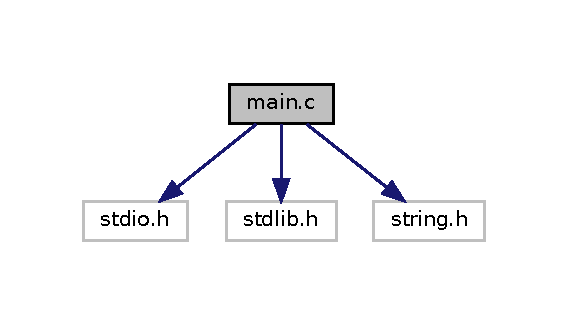
\includegraphics[width=273pt]{main_8c__incl}
\end{center}
\end{figure}
\subsection*{Functions}
\begin{DoxyCompactItemize}
\item 
int \hyperlink{main_8c_a0ddf1224851353fc92bfbff6f499fa97_a0ddf1224851353fc92bfbff6f499fa97}{main} (int argc, char $\ast$argv\mbox{[}$\,$\mbox{]})
\end{DoxyCompactItemize}


\subsection{Function Documentation}
\mbox{\Hypertarget{main_8c_a0ddf1224851353fc92bfbff6f499fa97_a0ddf1224851353fc92bfbff6f499fa97}\label{main_8c_a0ddf1224851353fc92bfbff6f499fa97_a0ddf1224851353fc92bfbff6f499fa97}} 
\index{main.\+c@{main.\+c}!main@{main}}
\index{main@{main}!main.\+c@{main.\+c}}
\subsubsection{\texorpdfstring{main()}{main()}}
{\footnotesize\ttfamily int main (\begin{DoxyParamCaption}\item[{int}]{argc,  }\item[{char $\ast$}]{argv\mbox{[}$\,$\mbox{]} }\end{DoxyParamCaption})}


\hypertarget{README_8md}{}\section{R\+E\+A\+D\+M\+E.\+md File Reference}
\label{README_8md}\index{R\+E\+A\+D\+M\+E.\+md@{R\+E\+A\+D\+M\+E.\+md}}

\hypertarget{template_8c}{}\section{template.\+c File Reference}
\label{template_8c}\index{template.\+c@{template.\+c}}
{\ttfamily \#include $<$stdio.\+h$>$}\newline
Include dependency graph for template.\+c\+:
\nopagebreak
\begin{figure}[H]
\begin{center}
\leavevmode
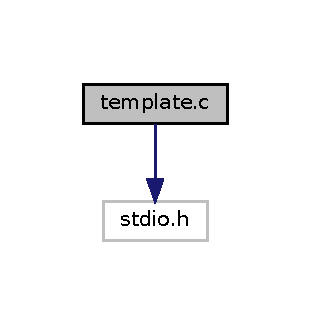
\includegraphics[width=149pt]{template_8c__incl}
\end{center}
\end{figure}
\subsection*{Functions}
\begin{DoxyCompactItemize}
\item 
int \hyperlink{template_8c_a0ddf1224851353fc92bfbff6f499fa97_a0ddf1224851353fc92bfbff6f499fa97}{main} (int argc, char $\ast$argv\mbox{[}$\,$\mbox{]})
\end{DoxyCompactItemize}


\subsection{Function Documentation}
\mbox{\Hypertarget{template_8c_a0ddf1224851353fc92bfbff6f499fa97_a0ddf1224851353fc92bfbff6f499fa97}\label{template_8c_a0ddf1224851353fc92bfbff6f499fa97_a0ddf1224851353fc92bfbff6f499fa97}} 
\index{template.\+c@{template.\+c}!main@{main}}
\index{main@{main}!template.\+c@{template.\+c}}
\subsubsection{\texorpdfstring{main()}{main()}}
{\footnotesize\ttfamily int main (\begin{DoxyParamCaption}\item[{int}]{argc,  }\item[{char $\ast$}]{argv\mbox{[}$\,$\mbox{]} }\end{DoxyParamCaption})}


\hypertarget{test__op_8c}{}\section{test\+\_\+op.\+c File Reference}
\label{test__op_8c}\index{test\+\_\+op.\+c@{test\+\_\+op.\+c}}
{\ttfamily \#include $<$stdio.\+h$>$}\newline
{\ttfamily \#include $<$string.\+h$>$}\newline
{\ttfamily \#include $<$unistd.\+h$>$}\newline
{\ttfamily \#include $<$stdlib.\+h$>$}\newline
{\ttfamily \#include $<$grp.\+h$>$}\newline
{\ttfamily \#include $<$pwd.\+h$>$}\newline
Include dependency graph for test\+\_\+op.\+c\+:
\nopagebreak
\begin{figure}[H]
\begin{center}
\leavevmode
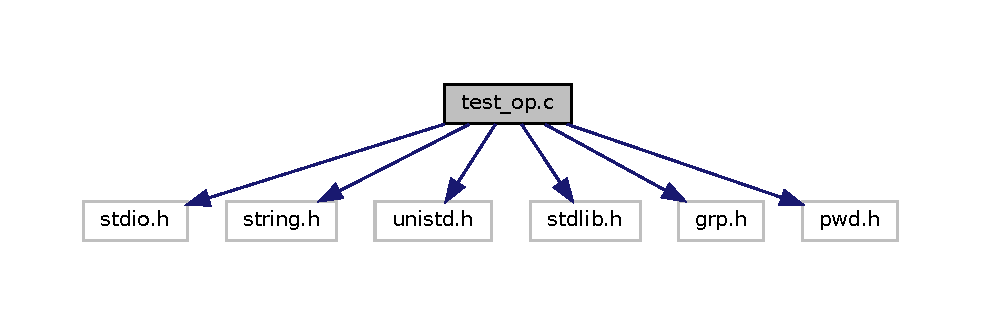
\includegraphics[width=350pt]{test__op_8c__incl}
\end{center}
\end{figure}
\subsection*{Functions}
\begin{DoxyCompactItemize}
\item 
int \hyperlink{test__op_8c_a0ddf1224851353fc92bfbff6f499fa97_a0ddf1224851353fc92bfbff6f499fa97}{main} (int argc, char $\ast$argv\mbox{[}$\,$\mbox{]})
\end{DoxyCompactItemize}


\subsection{Function Documentation}
\mbox{\Hypertarget{test__op_8c_a0ddf1224851353fc92bfbff6f499fa97_a0ddf1224851353fc92bfbff6f499fa97}\label{test__op_8c_a0ddf1224851353fc92bfbff6f499fa97_a0ddf1224851353fc92bfbff6f499fa97}} 
\index{test\+\_\+op.\+c@{test\+\_\+op.\+c}!main@{main}}
\index{main@{main}!test\+\_\+op.\+c@{test\+\_\+op.\+c}}
\subsubsection{\texorpdfstring{main()}{main()}}
{\footnotesize\ttfamily int main (\begin{DoxyParamCaption}\item[{int}]{argc,  }\item[{char $\ast$}]{argv\mbox{[}$\,$\mbox{]} }\end{DoxyParamCaption})}


%--- End generated contents ---

% Index
\backmatter
\newpage
\phantomsection
\clearemptydoublepage
\addcontentsline{toc}{chapter}{Index}
\printindex

\end{document}
